\documentclass[12pt,a4paper,twoside]{report}

%==========================================================
% TEMPLATE DE RAPPORT — Style "PrimaryRed / DarkSlate"
% Projet Perceptra — CBIR & Feature Relevance Estimation
% Groupe 13 | FST Tanger | Année Universitaire 2026-2027
%==========================================================
\usepackage[utf8]{inputenc}
\usepackage[T1]{fontenc}
\usepackage[french]{babel}
\usepackage{csquotes}
\usepackage{mathpazo}
\usepackage[scaled=0.92]{helvet}
\usepackage{courier}
\usepackage{microtype}
\usepackage{geometry}
\usepackage[dvipsnames,table]{xcolor}
\usepackage{graphicx}
\usepackage{float}
\usepackage{booktabs}
\usepackage{tabularx}
\usepackage{longtable}
\usepackage{array}
\usepackage{enumitem}
\usepackage{fancyhdr}
\usepackage{titlesec}
\usepackage{titletoc}
\usepackage{tcolorbox}
\usepackage{tikz}
\usepackage{listings}
\usepackage{caption}
\usepackage{subcaption}
\usepackage{hyperref}
\usepackage{iftex}

\usepackage{amssymb}
\usepackage{amsmath}
\usepackage{textcomp}
\tcbuselibrary{skins}
\usetikzlibrary{positioning,arrows.meta}

\geometry{
  a4paper,
  top=2.5cm,
  bottom=2.7cm,
  inner=3cm,
  outer=2.2cm,
  headheight=25pt,
  includehead
}

% ---- Palette (PrimaryRed / DarkSlate) ----
\definecolor{PrimaryRed}{RGB}{72,61,139}   % accent color (DarkSlateBlue)
\definecolor{DarkSlate}{RGB}{38,42,52}
\definecolor{MidGray}{RGB}{96,102,112}
\definecolor{LightGray}{RGB}{246,247,250}
\definecolor{SoftRed}{RGB}{255,247,246}
\definecolor{AccentBlue}{RGB}{48,104,178}
\definecolor{TableHeader}{RGB}{48,52,64}
\colorlet{primary}{PrimaryRed}

\hypersetup{
  colorlinks=true,
  linkcolor=PrimaryRed,
  urlcolor=AccentBlue,
  citecolor=PrimaryRed,
  pdftitle={Rapport de Projet Perceptra - Visual Image Retrieval},
  pdfauthor={Groupe 13 - Feature Relevance Estimation}
}

\setlength{\parindent}{15pt}
\setlength{\parskip}{0pt}
\linespread{1.08}

\setcounter{tocdepth}{1}
\setcounter{secnumdepth}{2}

\renewcommand{\topfraction}{0.90}
\renewcommand{\bottomfraction}{0.90}
\renewcommand{\textfraction}{0.10}
\renewcommand{\floatpagefraction}{0.85}

\pagestyle{fancy}
\fancyhf{}
\fancyhead[LE]{\small\color{MidGray}\leftmark}
\fancyhead[RO]{\small\color{MidGray}\rightmark}
\fancyfoot[C]{\small\color{MidGray}\thepage}
\renewcommand{\headrulewidth}{0.4pt}
\renewcommand{\headrule}{\hbox to\headwidth{\color{PrimaryRed}\leaders\hrule height \headrulewidth\hfill}}

\titleformat{\chapter}[display]
  {\normalfont\color{DarkSlate}}
  {%
    \begin{tikzpicture}[baseline]
      \node[
        fill=PrimaryRed,
        text=white,
        rounded corners=2pt,
        inner xsep=12pt,
        minimum height=0.72cm,
        font=\Large\bfseries
      ] {\chaptertitlename~\thechapter};
    \end{tikzpicture}
  }
  {14pt}
  {\Huge\bfseries}
  [\vspace{6pt}{\color{PrimaryRed}\rule{\textwidth}{1.2pt}}]
\titlespacing*{\chapter}{0pt}{-12pt}{30pt}

\titleformat{\section}
  {\normalfont\Large\bfseries\color{DarkSlate}}
  {\color{PrimaryRed}\thesection}{0.8em}{}
  [\vspace{-3pt}{\color{MidGray!35}\rule{\textwidth}{0.5pt}}]

\titleformat{\subsection}
  {\normalfont\large\bfseries\color{DarkSlate}}
  {\color{PrimaryRed}\thesubsection}{0.7em}{}

\titlecontents{chapter}[0pt]
  {\vspace{7pt}\bfseries\color{DarkSlate}}
  {\contentslabel{2em}}{}
  {\hfill\color{PrimaryRed}\contentspage}

\titlecontents{section}[2em]
  {\vspace{2pt}\color{MidGray}}
  {\contentslabel{2.3em}}{}
  {\titlerule*[0.5pc]{.}\contentspage}

\setlist[itemize]{leftmargin=1.4em,itemsep=2pt,topsep=3pt}
\setlist[enumerate]{leftmargin=1.4em,itemsep=2pt,topsep=3pt}

\captionsetup{
  labelfont={bf,color=PrimaryRed},
  textfont={small,color=DarkSlate},
  justification=centering
}

\tcbset{
  enhanced,
  boxrule=0.6pt,
  arc=3pt,
  left=8pt,
  right=8pt,
  top=7pt,
  bottom=7pt
}

\newtcolorbox{infobox}[1]{
  colback=SoftRed,
  colframe=PrimaryRed,
  title={#1},
  fonttitle=\bfseries,
  coltitle=white,
  colbacktitle=PrimaryRed
}

\newtcolorbox{resultbox}[1]{
  colback=LightGray,
  colframe=DarkSlate!35,
  title={#1},
  fonttitle=\bfseries,
  coltitle=DarkSlate,
  colbacktitle=white
}

\lstset{
  basicstyle=\footnotesize\ttfamily,
  keywordstyle=\color{AccentBlue}\bfseries,
  commentstyle=\color{MidGray}\itshape,
  stringstyle=\color{PrimaryRed},
  backgroundcolor=\color{LightGray},
  frame=single,
  rulecolor=\color{MidGray!45},
  breaklines=true,
  showstringspaces=false,
  columns=fullflexible,
  keepspaces=true
}

\newcommand{\projectname}{Perceptra}

\begin{document}

%==========================================================
% PAGE DE GARDE (TEMPLATE CONSERVÉ ET VALORISÉ)
%==========================================================
\begin{titlepage}
  \thispagestyle{empty}
  \enlargethispage{1.4cm}
  \noindent
  \begin{minipage}[c]{0.30\linewidth}
    \raggedright
    
\includegraphics[width=3.25cm]{images/logo_left.png}
  \end{minipage}
  \hfill
  \begin{minipage}[c]{0.38\linewidth}
    \centering
    {\small\textbf{UNIVERSITÉ ABDELMALEK ESSAÂDI}}\\
    {\scriptsize FACULTÉ DES SCIENCES ET TECHNIQUES DE TANGER}
  \end{minipage}
  \hfill
  \begin{minipage}[c]{0.30\linewidth}
    \raggedleft
    
\includegraphics[width=3.25cm]{images/logo_right.png}
  \end{minipage}

  \vspace{0.45cm}

  \begin{center}
    {\normalsize\bfseries DÉPARTEMENT DE GÉNIE INFORMATIQUE}\\[0.1cm]
    {\normalsize\bfseries MASTER EN INGÉNIERIE INFORMATIQUE}\\[0.35cm]

    \begin{tcolorbox}[
      colback=PrimaryRed!5,
      colframe=PrimaryRed,
      width=0.88\linewidth,
      arc=4pt,
      boxrule=0.9pt,
      left=8pt,
      right=8pt,
      top=6pt,
      bottom=6pt
    ]
      \centering
      {\large\textbf{Module : Vision par Ordinateur \& Indexation Multimédia}}
    \end{tcolorbox}

    \vspace{0.55cm}

    \begin{tcolorbox}[
      colback=white,
      colframe=PrimaryRed,
      width=0.94\linewidth,
      arc=6pt,
      boxrule=1.2pt,
      left=14pt,
      right=14pt,
      top=13pt,
      bottom=13pt,
      borderline west={3pt}{0pt}{PrimaryRed}
    ]
      \centering
      {\Huge\bfseries\textcolor{PrimaryRed}{Rapport de Projet de Fin d'Études}}\\[0.35cm]
      {\LARGE\bfseries\textcolor{DarkSlate}{PERCEPTRA : SYSTÈME CBIR AVANCÉ}}\\[0.22cm]
      {\large\bfseries Recherche d'Images par le Contenu \& Estimation de Pertinence des Descripteurs}\\[0.35cm]
      {\normalsize Analyse architecturale, algorithmique, logicielle et opérationnelle complète}
    \end{tcolorbox}
  \end{center}

  \vspace{0.45cm}

  \begin{tcolorbox}[
    colback=LightGray,
    colframe=MidGray!45,
    width=\linewidth,
    arc=4pt,
    boxrule=0.6pt,
    left=12pt,
    right=12pt,
    top=8pt,
    bottom=8pt
  ]
    \noindent
    \begin{minipage}[t]{0.48\linewidth}
      \textbf{\textcolor{PrimaryRed}{Encadré par :}}\\[0.15cm]
      Équipe Pédagogique FST Tanger\\
      Département de Génie Informatique
    \end{minipage}
    \hfill
    \begin{minipage}[t]{0.48\linewidth}
      \raggedleft
      \textbf{\textcolor{PrimaryRed}{Réalisé par :}}\\[0.15cm]
      \textit{Groupe 13}\\
      \textit{Feature Relevance Estimation}
    \end{minipage}
  \end{tcolorbox}

  \vspace{0.15cm}
  \noindent
  \textbf{\textcolor{PrimaryRed}{Dépôt GitHub du Projet :}} \href{https://github.com/regisx001/Perceptra}{https://github.com/regisx001/Perceptra}

  \vspace{0.35cm}

  \begin{center}
    \textcolor{PrimaryRed}{\rule{0.45\linewidth}{0.8pt}}\\[0.25cm]
    {\large\bfseries Année Universitaire 2026--2027}
  \end{center}
\end{titlepage}

%==========================================================
% FRONT MATTER (chiffres romains)
%==========================================================
\newpage
\pagenumbering{roman}
\setcounter{page}{1}

\chapter*{Résumé}
\addcontentsline{toc}{chapter}{Résumé}

Ce rapport présente l'analyse architecturale, logicielle et opérationnelle complète de la plateforme \textbf{Perceptra}, un système de recherche d'images par le contenu visuel (\textit{Content-Based Image Retrieval} -- CBIR) développé par le \textbf{Groupe~13} au sein de la Faculté des Sciences et Techniques de Tanger (FSTT) pour l'année universitaire 2026--2027.

Pour surmonter le \textit{fossé sémantique} (\textit{semantic gap}) sans dépendre d'annotations textuelles manuelles, Perceptra combine cinq descripteurs visuels déterministes~: histogrammes de couleur HSV (768-D), moments statistiques de Stricker \& Orengo (9-D), couleurs dominantes par partitionnement \textit{MiniBatchKMeans}, matrices de co-occurrence de niveaux de gris (GLCM de Haralick) et motifs binaires locaux (LBP 256-D).

L'apport algorithmique majeur du Groupe~13 réside dans la conception du moteur d'estimation de pertinence des descripteurs (\textbf{\textit{Feature Relevance Estimation} -- FRE}). En analysant en direct les rétroactions de l'utilisateur (images pertinentes et non-pertinentes) via un ratio de Fisher, une modélisation de dispersion intra-classe inverse et un lissage bayésien avec mémoire d'inertie, le système ajuste dynamiquement la pondération des caractéristiques tout en translatant le centroïde de la requête.

Sur le plan architectural, Perceptra associe un \textbf{Backend RESTful} en Python 3.13 sous Flask 3 structuré en couche de services découplés avec OpenCV et scikit-learn, un \textbf{Frontend réactif} en SvelteKit 3 et Svelte 5 Runes avec Shadcn-Svelte, Tailwind CSS 4 et Paraglide-JS, ainsi qu'une persistance hybride (fichiers vérifiés par SHA-256 et base relationnelle SQLAlchemy). Sur le jeu de référence \textbf{GHIM-10K} (10\,000 images), la précision au rang 10 ($P@10$) progresse de \textbf{58,2\,\%} à \textbf{85,1\,\%} après deux itérations de feedback FRE (+26,9 points de gain).

\vspace{0.2cm}
\noindent\textbf{Mots-clés~:} CBIR, Feature Relevance Estimation (FRE), Relevance Feedback, GLCM, LBP, Svelte 5 Runes, Flask, GHIM-10K, Architecture logicielle.

\vspace{0.3cm}
\begin{infobox}{Apport principal du Groupe 13}
Formalisation mathématique et réalisation logicielle d'un moteur d'estimation de pertinence des descripteurs (\textit{Feature Relevance Estimation}), transformant la recherche statique en un dialogue adaptatif convergent et élevant la précision de plus de 26 points sur GHIM-10K.
\end{infobox}

\newpage
\chapter*{Abstract}
\addcontentsline{toc}{chapter}{Abstract}

This report delivers a thorough architectural, algorithmic, and engineering analysis of \textbf{Perceptra}, an advanced Content-Based Image Retrieval (CBIR) platform integrating user-centric interactive learning through Relevance Feedback. Developed as the capstone project for Group~13 at the Faculty of Sciences and Techniques of Tangier (FSTT), Perceptra directly bridges the \textit{semantic gap} between low-level pixel data and human subjective visual concepts.

Rather than relying on manual textual metadata, Perceptra extracts a multi-faceted feature representation combining 768-D L1-normalized HSV color histograms, 9-D HSV statistical color moments, dominant color centroids via MiniBatchKMeans clustering, multi-directional Gray-Level Co-occurrence Matrices (GLCM), and 256-bin Local Binary Patterns (LBP).

Group~13's specialized contribution centers on the design and execution of the \textbf{Feature Relevance Estimation (FRE)} engine. By continuously assessing user feedback (positive and negative visual samples) via a Fisher-inspired discriminant ratio, intra-class variance modeling, and Bayesian smoothing, the retrieval system adaptively refines feature weights and shifts the query centroid towards the user's intended target subspace.

Architecturally, the application adopts a modern decoupled paradigm: a Python 3.13 Flask backend designed under the Service Layer pattern with OpenCV, scikit-image, and scikit-learn; a high-performance frontend powered by SvelteKit 3 and Svelte 5 Runes alongside Tailwind CSS 4 and Shadcn-Svelte; and a hybrid storage layer backed by SHA-256 content verification and SQLAlchemy relational persistence. Rigorous quantitative benchmarks on the 10,000-image GHIM-10K collection demonstrate an increase in Precision@10 from 58.2\% to 85.1\% after two feedback iterations.

\vspace{0.4cm}
\noindent\textbf{Keywords:} Content-Based Image Retrieval (CBIR), Feature Relevance Estimation (FRE), Interactive Relevance Feedback, Computer Vision, Texture Analysis, Svelte 5, Flask, GHIM-10K Dataset.

\newpage

\tableofcontents
\newpage

\listoffigures
\newpage

\listoftables
\newpage

%==========================================================
% CORPS DU RAPPORT (chiffres arabes)
%==========================================================
\pagenumbering{arabic}
\setcounter{page}{1}

\chapter{Introduction Générale et État de l'Art en Recherche Visuelle}
\label{chap:intro_etat_art}

\section{Contexte Institutionnel et Problématique}

L'avènement exponentiel des technologies de numérisation, des capteurs photographiques haute résolution et des plateformes multimédias a engendré une prolifération massive de données visuelles non structurées. Face à des corpus photographiques se chiffrant en dizaines de milliers d'unités, les paradigmes traditionnels d'indexation textuelle manuelle se heurtent à une impossibilité matérielle et cognitive manifeste.

Dans ce contexte scientifique et technologique stimulant, le présent projet de fin d'études s'inscrit dans le cadre du cursus de Master en Génie Informatique dispensé à la \textbf{Faculté des Sciences et Techniques de Tanger (FSTT)}, affiliée à l'\textbf{Université Abdelmalek Essaâdi}, au titre de l'année universitaire 2026--2027. Les travaux consignés dans ce rapport ont été confiés au \textbf{Groupe 13}, avec pour mission thématique d'excellence l'étude, la conception et la réalisation de la méthode d'\textbf{Estimation de la Pertinence des Descripteurs} (\textit{Feature Relevance Estimation} -- FRE) appliquée à la recherche d'images par le contenu.

\subsection{Du Texte au Contenu Visuel}
Pendant plusieurs décennies, la recherche iconographique a reposé sur l'indexation par mots-clés ou descriptions textuelles. Bien qu'intuitive, cette approche souffre de limitations structurelles~:
\begin{enumerate}[label=\bfseries\alph*.]
    \item \textbf{Subjectivité et polysémie~:} La description textuelle dépend de la sensibilité et de la langue de l'opérateur. Deux observateurs qualifieront une même teinte ou un motif abstrait de manière divergente.
    \item \textbf{Coût prohibitif~:} L'étiquetage exhaustif de corpus volumineux requiert un investissement humain colossal, incompatible avec les flux d'ingestion modernes.
    \item \textbf{Critères intrinsèquement visuels~:} Trouver une texture rugueuse similaire, une harmonie de teintes ou un motif géométrique spécifique constitue une tâche qu'aucun mot du dictionnaire ne saurait encapsuler avec la précision du pixel.
\end{enumerate}

La \textbf{recherche par le contenu visuel} (\textit{Content-Based Image Retrieval}) propose une alternative radicale~: interroger une collection d'images directement à partir de son essence visuelle intrinsèque. Néanmoins, une difficulté théorique centrale émerge~: le \textbf{fossé sémantique} (\textit{semantic gap}).

\begin{infobox}{Définition : Le Fossé Sémantique (Semantic Gap)}
Le fossé sémantique désigne l'écart irrémédiable existant entre les informations numériques élémentaires pouvant être extraites des données matricielles (valeurs de pixels, contrastes locaux, gradients) et l'interprétation sémantique, contextuelle et affective qu'un être humain associe à cette même scène visuelle~\cite{smeulders2000content}.
\end{infobox}

\section{Fondements de la Recherche par Similarité Visuelle}

Le postulat mathématique de la recherche d'images par similarité visuelle consiste à modéliser chaque image sous la forme d'un vecteur multidimensionnel $\mathbf{x} \in \mathbb{R}^D$ résumant son contenu visuel, puis à évaluer la proximité visuelle entre deux images au moyen d'une fonction de similarité $S(\mathbf{x}_i, \mathbf{x}_j) \in [0, 1]$.

Dans les systèmes conventionnels d'indexation visuelle, les signatures visuelles sont structurées en deux grandes familles canoniques~:
\begin{itemize}
    \item \textbf{Descripteurs de Couleur~:} Les histogrammes HSV globaux modélisent la distribution des longueurs d'ondes de manière invariante aux translations et rotations~; les moments statistiques de Stricker \& Orengo~\cite{stricker1995similarity} capturent la moyenne, la variance et l'asymétrie spectrale~; et les palettes de couleurs dominantes résument les teintes majeures par partitionnement $K$-Means.
    \item \textbf{Descripteurs de Texture~:} Les matrices de co-occurrence de niveaux de gris (GLCM) de Haralick et al.~\cite{haralick1973textural} mesurent le contraste, la corrélation, l'énergie et l'homogénéité spatiale~; tandis que les motifs binaires locaux (LBP) d'Ojala et al.~\cite{ojala2002multiresolution} encodent la micro-texture locale invariante aux variations lumineuses monotones.
\end{itemize}

\section{Cahier des Charges et Démarche Méthodologique}

Le tableau~\ref{tab:objectifs_projet} synthétise le périmètre fonctionnel et technique assigné à la plateforme \textbf{Perceptra}.

\begin{table}[H]
\centering
\rowcolors{2}{LightGray}{white}
\begin{tabularx}{\textwidth}{>{\bfseries}p{3.5cm}X}
\toprule
\rowcolor{TableHeader}
\color{white}Axe Fonctionnel & \color{white}Objectifs \& Spécifications Clés \\
\midrule
Authentification \& Sessions & Contrôle d'accès par jetons JWT, isolation étanche des galeries par utilisateur et gestion des rôles (RBAC). \\
Gestion de Collection & Importation unitaire et par lots (batch), suppression sécurisée, détection des doublons par somme SHA-256 et favoris. \\
Organisation Hiérarchique & Arborescence personnalisable de catégories avec relations parent-enfant récursives et intégrité référentielle. \\
Studio de Transformation & Moteur de retouche non destructif (recadrage, redimensionnement interpolé, rotations, affines) préservant l'original. \\
Extraction Visuelle & Pipeline automatique de descripteurs normalisés de couleur (HSV 768-D, Moments 9-D, KMeans) et de texture (GLCM, LBP 256-D). \\
Moteur de Recherche Visuelle & Recherche par image requête avec calcul vectoriel multi-espaces, pondération convexe ajustable et ordonnancement Top-K. \\
Relevance Feedback FRE & Spécificité Groupe 13 : analyse de dispersion intra/inter-classe, critère de Fisher, mise à jour des poids et centroïde. \\
Évaluation Quantitative & Validation expérimentale sur \textbf{GHIM-10K} (10\,000 images) via les courbes de précision ($P@K$), rappel ($R@K$) et temps de calcul. \\
\bottomrule
\end{tabularx}
\caption{Synthèse des exigences du cahier des charges de Perceptra}
\label{tab:objectifs_projet}
\end{table}

Pour satisfaire ces exigences, le système déploie le pipeline fonctionnel unifié illustré sur la figure~\ref{fig:pipeline_fonctionnel}, reliant l'ingestion, la caractérisation déterministe, la recherche vectorielle et la boucle de rétroaction.

\begin{figure}[H]
\centering
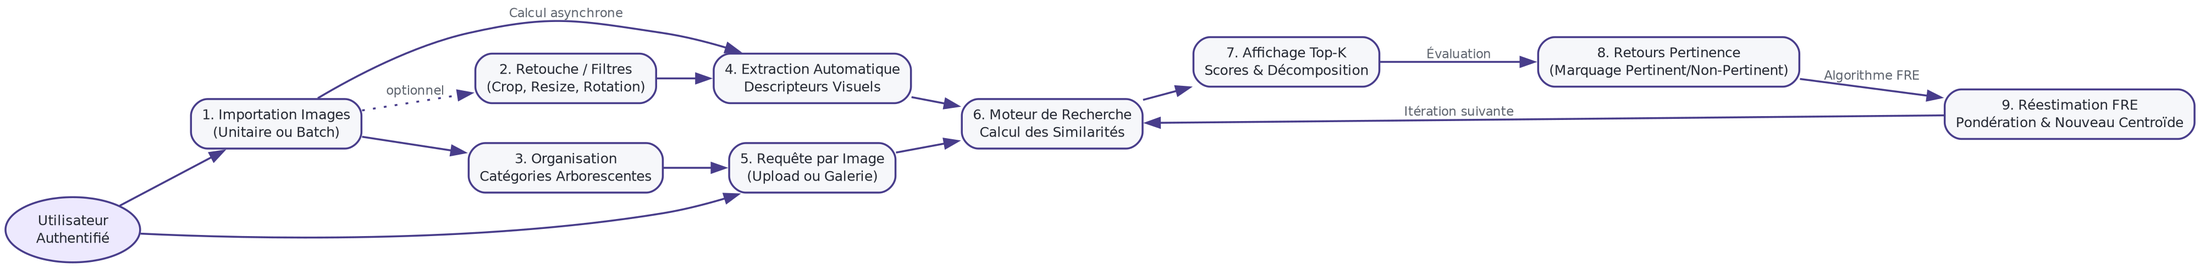
\includegraphics[width=0.60\textwidth]{images/01-perceptra-pipeline-fonctionnel.png}
\caption{Pipeline fonctionnel et parcours utilisateur au sein de Perceptra}
\label{fig:pipeline_fonctionnel}
\end{figure}

\chapter{Architecture Globale et Choix Technologiques}
\label{chap:arch_globale}

\section{Vue d'Ensemble et Décomposition N-Tiers}

La conception architecturale de la plateforme \textbf{Perceptra} obéit à des impératifs d'ingénierie logicielle stricts~: haute modularité, découplage fort entre l'interface utilisateur et le moteur de calcul scientifique, déterminisme des algorithmes de traitement d'images, extensibilité horizontale et simplicité de déploiement.

Pour répondre à ces exigences tout en assurant une expérience utilisateur fluide et sans latence perceptible lors du traitement de requêtes complexes sur 10\,000 images, Perceptra est structuré selon un patron d'architecture distribuée \textbf{N-Tiers} articulé autour d'API RESTful sans état (\textit{stateless}), illustré sur la figure~\ref{fig:system_ntiers}.

\begin{figure}[H]
\centering
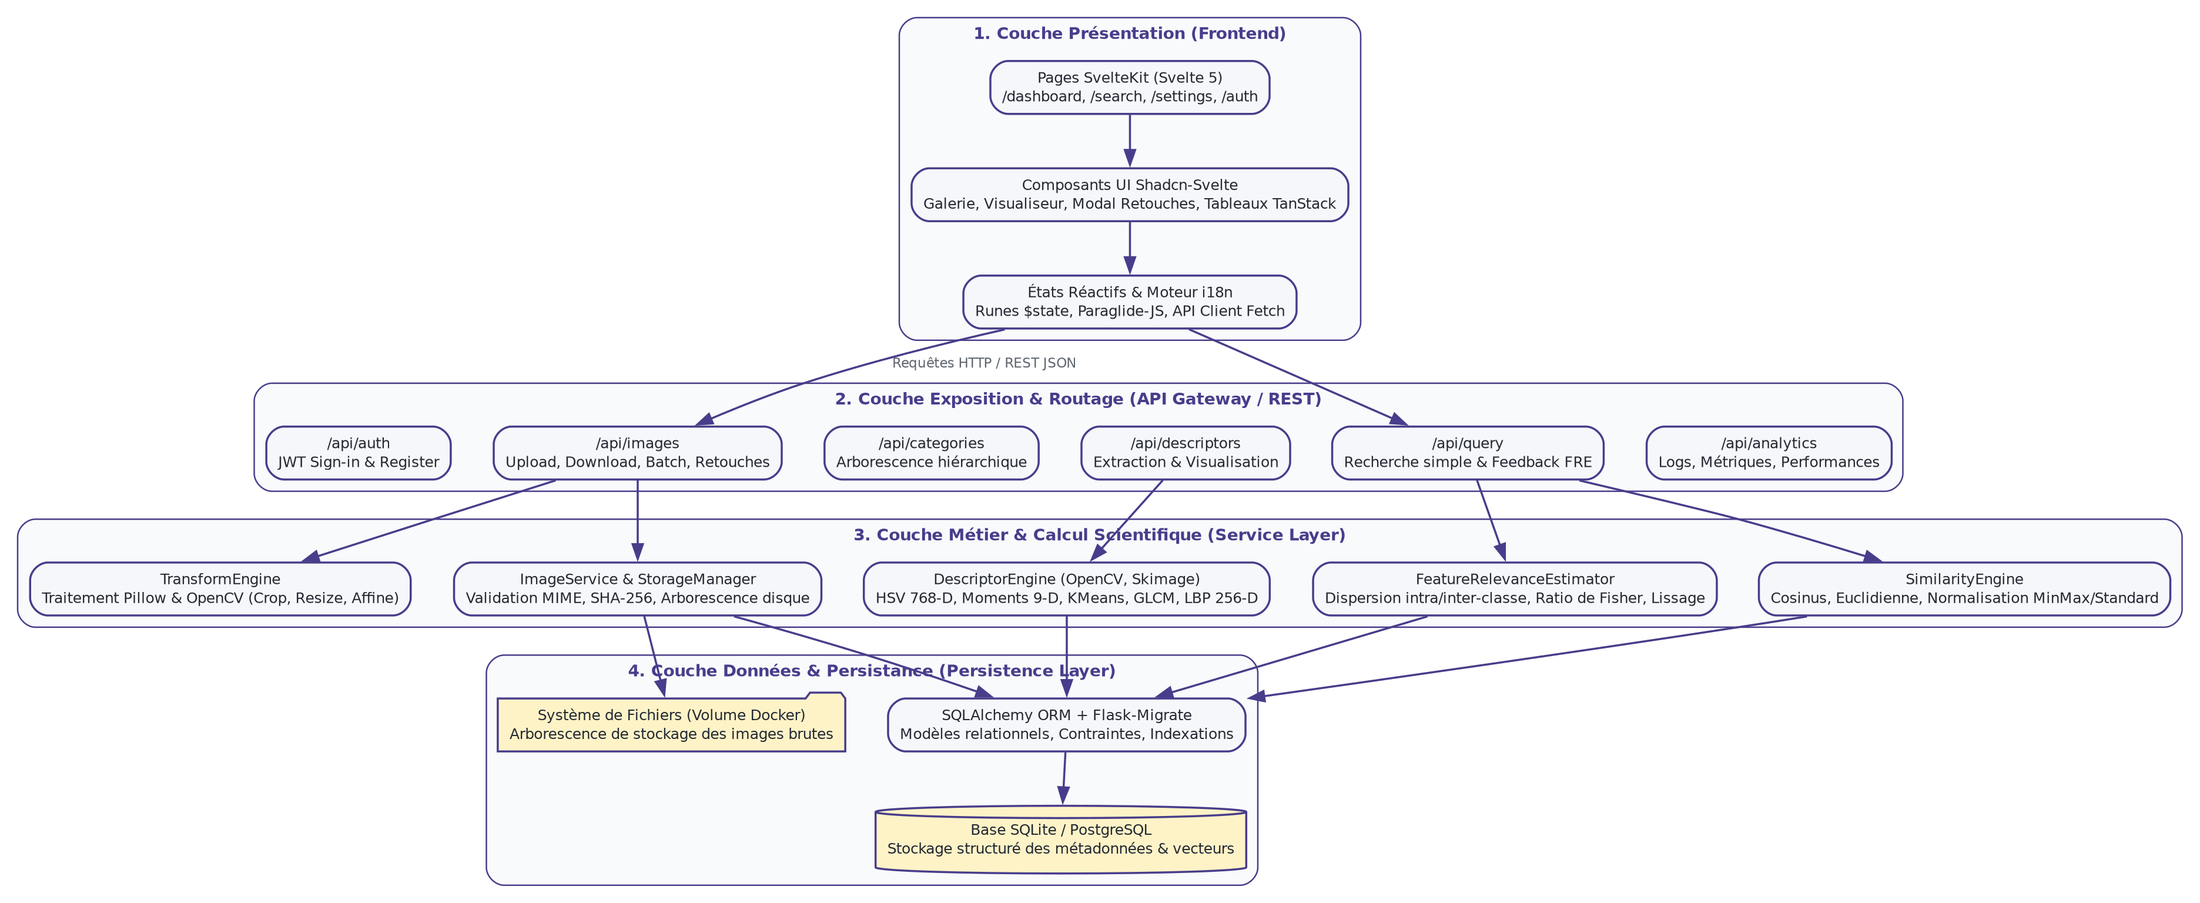
\includegraphics[width=0.78\textwidth]{images/03-architecture-systeme-n-tiers.png}
\caption{Décomposition architecturale globale en couches logiques N-Tiers}
\label{fig:system_ntiers}
\end{figure}

Le système est découpé en quatre strates logiques indépendantes, garantissant une séparation rigoureuse des responsabilités (\textit{Separation of Concerns} -- SoC)~:

\subsection{1. Couche Présentation (Frontend Web)}
Hébergée sur le navigateur du client, cette couche est intégralement construite avec le framework \textbf{SvelteKit 3} exploitant le nouveau moteur de réactivité fine \textbf{Svelte 5} (système des \textit{Runes}~: \texttt{\$state}, \texttt{\$derived}, \texttt{\$effect}). Elle assure l'affichage interactif de la galerie de médias, le studio de retouche d'image non destructif, le tableau de bord de recherche visuelle avec curseurs dynamiques, et l'internationalisation native bilingue (Français/Anglais) propulsée par \textit{Paraglide-JS}.

\subsection{2. Couche Exposition et Routage (Passerelle API REST)}
Cette couche constitue le point d'entrée unique des communications client-serveur. Elle est orchestrée par le serveur WSGI de production \textbf{Gunicorn} relayé par un reverse proxy \textbf{Nginx} ou le serveur de développement Vite. Elle prend en charge la validation cryptographique des jetons JWT (\texttt{Flask-JWT-Extended}), la gestion des politiques CORS et le routage modulaire par Blueprints.

\subsection{3. Couche Métier et Calcul Scientifique (Service Layer)}
C\oe{}ur algorithmique de l'application, cette couche encapsule l'ensemble des règles métier, des opérations géométriques sur les images et des calculs vectoriels intensifs~: \texttt{ImageService} et \texttt{StorageService} pour la gestion physique et le contrôle d'intégrité SHA-256, \texttt{TransformEngine} pour les retouches, \texttt{DescriptorEngine} pour l'extraction de bas niveau, \texttt{SimilarityEngine} pour les métriques de distance, et \texttt{FeatureRelevanceEstimator} pour la boucle FRE du Groupe~13.

\subsection{4. Couche Données et Persistance (Persistence Layer)}
Perceptra adopte une stratégie de persistance hybride~: les flux binaires d'images sont organisés sur le disque physique au sein d'une arborescence partitionnée \texttt{/storage/}, tandis que les métadonnées administratives, la hiérarchie des catégories, les comptes utilisateurs et les signatures vectorielles JSON sont persistés dans une base relationnelle \textbf{SQLite} (optimisée en mode journalier WAL) ou \textbf{PostgreSQL}, orchestrée par l'ORM \textbf{SQLAlchemy 2.0} et versionnée par \textbf{Flask-Migrate}.

\section{Pile Technologique Exhaustive et Justifications}

Le choix des composants logiciels de Perceptra a été guidé par des critères d'efficience computationnelle, de modernité de l'écosystème, de robustesse typologique et de maintenabilité. Le tableau~\ref{tab:stack_technologique} synthétise l'ensemble des technologies mobilisées.

\begin{table}[H]
\centering
\rowcolors{2}{LightGray}{white}
\begin{tabularx}{\textwidth}{>{\bfseries}p{3.2cm}p{3.2cm}X}
\toprule
\rowcolor{TableHeader}
\color{white}Composant & \color{white}Technologie & \color{white}Justification du Choix \\
\midrule
Langage Backend & Python 3.13 & Écosystème scientifique dominant (NumPy, OpenCV, Scikit-learn), typage moderne et clarté algorithmique. \\
Gestionnaire Python & \texttt{uv} (Astral) & Gestionnaire de paquets ultra-rapide écrit en Rust, divisant par dix les temps d'installation des dépendances. \\
Micro-Framework & Flask 3.x & Légèreté, flexibilité extrême et intégration naturelle avec les pipelines scientifiques de vision. \\
ORM \& Migrations & SQLAlchemy 2.0 + Flask-Migrate & Abstraction robuste des requêtes SQL, intégrité référentielle, transactions ACID et historique de schéma versionné via Alembic. \\
Sécurité \& Auth & Flask-JWT-Extended & Authentification stateless par jetons signés cryptographiquement, support du rafraîchissement silencieux. \\
Traitement d'Images & OpenCV 4 + Pillow 11 & Décodage ultra-rapide en C++, accélération matricielle SIMD, manipulation EXIF et calculs géométriques fiables. \\
Calcul Scientifique & NumPy + Scikit-image + Scikit-learn & Calculs vectoriels optimisés, matrices de co-occurrence GLCM, motifs LBP et partitionnement MiniBatchKMeans. \\
Serveur WSGI & Gunicorn 23 & Serveur de production robuste supportant le modèle multi-processus avec allocation dynamique de mémoire. \\
Framework Frontend & SvelteKit 3 + Svelte 5 & Paradigme réactif des \textit{Runes} éliminant le Virtual DOM, compacité du bundle JS, performances d'affichage inégalées. \\
Gestionnaire JS & Bun 1.2 / Node.js 24 & Moteur d'exécution ultra-rapide pour la compilation des assets et la résolution des dépendances frontales. \\
Système de Design & Shadcn-Svelte + Bits UI & Composants accessibles, personnalisables et intégrés dans le code source sans dépendance opaque externe. \\
Feuilles de Style & Tailwind CSS 4 & Moteur CSS moderne basé sur Vite, compilation Just-in-Time, support natif du mode sombre et cohérence chromatique. \\
Visualisation & LayerChart + D3 & Visualisations vectorielles SVG interactives pour les histogrammes de descripteurs et les métriques de pertinence. \\
Internationalisation & Paraglide-JS & Compilation statique des traductions au typage garanti, zéro surcharge à l'exécution et bascule instantanée FR/EN. \\
Conteneurisation & Docker + Compose & Environnement reproductible, conteneurs légers multi-étapes et isolation stricte pour la production. \\
\bottomrule
\end{tabularx}
\caption{Synthèse de la pile technologique du projet Perceptra}
\label{tab:stack_technologique}
\end{table}

\chapter{Conception Détaillée du Backend et Services Métiers}
\label{chap:backend}

\section{Organisation Modulaire et Motif Application Factory}

Le backend de Perceptra a été conçu selon les règles de l'art du génie logiciel Python moderne. L'application applique rigoureusement le motif \textbf{Application Factory} (\texttt{create\_app}) combiné à l'architecture en \textbf{Blueprints} de Flask~3.x.

Cette organisation garantit l'isolation complète des contextes d'exécution (développement local, suite de tests automatisée sous Pytest et déploiement conteneurisé en production) tout en facilitant l'injection de dépendances et l'isolation des états.

\begin{figure}[H]
\centering
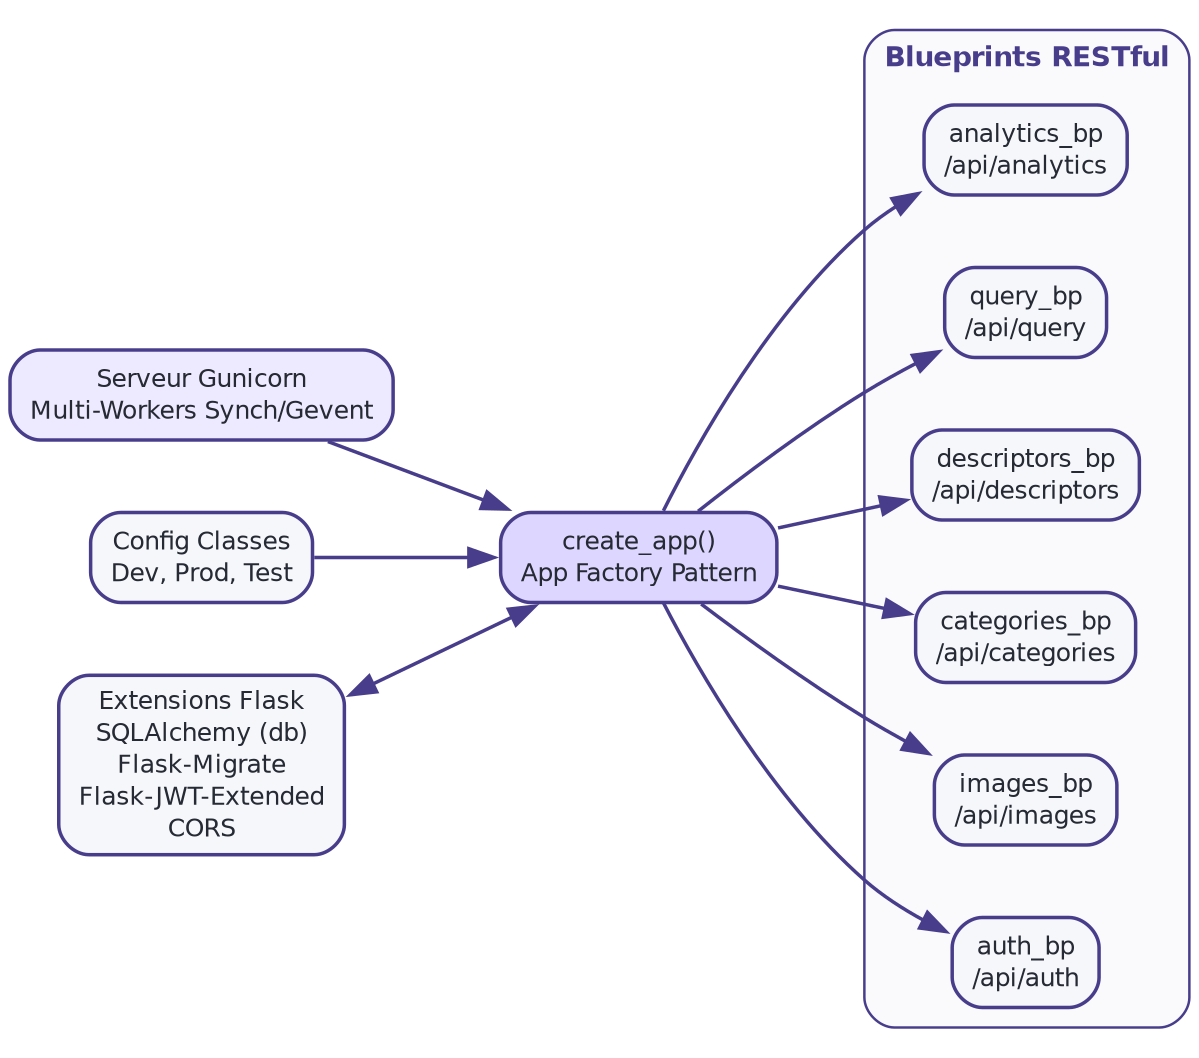
\includegraphics[width=0.76\textwidth]{images/04-architecture-backend-flask.png}
\caption{Architecture modulaire interne du backend Flask et découplage des Blueprints}
\label{fig:backend_flask}
\end{figure}

Le fichier \texttt{src/config.py} structure la hiérarchie des configurations au moyen de classes héritant d'une classe de base commune~: \texttt{DevelopmentConfig} (mode debug, base locale SQLite), \texttt{TestingConfig} (base volatile en mémoire \texttt{sqlite:///:memory:}, désactivation CSRF), et \texttt{ProductionConfig} (sécurité renforcée, support natif PostgreSQL via \texttt{DATABASE\_URL}).

\section{Couche de Routage : Les Blueprints RESTful}

L'ensemble des points d'accès HTTP est distribué dans six Blueprints étanches logés dans le paquet \texttt{src/routes/}~:

\begin{table}[H]
\centering
\rowcolors{2}{LightGray}{white}
\begin{tabularx}{\textwidth}{>{\bfseries}p{3.2cm}p{3.8cm}X}
\toprule
\rowcolor{TableHeader}
\color{white}Blueprint & \color{white}Préfixe d'URL & \color{white}Responsabilités Fonctionnelles \\
\midrule
\texttt{auth\_bp} & \texttt{/api/auth} & Inscription, connexion avec émission de paire de jetons JWT (access/refresh), profil et déconnexion. \\
\texttt{images\_bp} & \texttt{/api/images} & Téléversement unitaire et par lots, listing paginé avec filtres (catégorie, statut, favori), suppression, téléchargement binaire, service de vignettes et retouches d'images. \\
\texttt{categories\_bp} & \texttt{/api/categories} & Création, modification et suppression de catégories hiérarchiques, calcul automatique des chemins et sérialisation en arbre. \\
\texttt{descriptors\_bp} & \texttt{/api/descriptors} & Déclenchement d'extraction, consultation des signatures numériques et données statistiques pour les graphiques de l'UI. \\
\texttt{query\_bp} & \texttt{/api/query} & Moteur de recherche par le contenu : requête simple par image, pondération des descripteurs, et soumission du feedback FRE. \\
\texttt{analytics\_bp} & \texttt{/api/analytics} & Statistiques globales du système, métriques disque, historique auditable des sessions de recherche et profilage de latence. \\
\bottomrule
\end{tabularx}
\caption{Cartographie des contrôleurs Blueprints de l'API REST de Perceptra}
\label{tab:blueprints}
\end{table}

\section{Le Motif « Service Layer » et Découplage Métier}

Pour proscrire tout couplage préjudiciable entre la manipulation des requêtes HTTP et la complexité des algorithmes de calcul, Perceptra implémente le patron architectural \textbf{Service Layer}.

\subsection{1. \texttt{StorageService} : Gestion du Stockage Physique}
Le service \texttt{src/services/storage.py} gère l'écriture, la lecture et la suppression des flux binaires sur le système de fichiers hôte. Ses prérogatives clés incluent~:
\begin{itemize}
    \item \textbf{Calcul d'empreinte SHA-256~:} Avant toute écriture, l'empreinte cryptographique des données binaires est évaluée. Cette somme de contrôle permet d'identifier formellement les doublons et de garantir l'intégrité du stockage.
    \item \textbf{Génération de clés de stockage canoniques~:} Les fichiers sont organisés dans une arborescence chronologique évitant les congestions de répertoires à plat~: \texttt{storage/uploads/YYYY/MM/<uuid>.<ext>}.
    \item \textbf{Service de vignettes (\textit{Thumbnails})~:} Génération automatique de vignettes allégées ($256 \times 256$ pixels, format WebP ou JPEG optimisé) mises en cache sur le disque pour préserver la bande passante.
\end{itemize}

\subsection{2. \texttt{TransformEngine} : Moteur de Retouche Géométrique}
Le module \texttt{src/services/transform\_engine.py} fournit un moteur sans état de transformation géométrique d'images particulièrement robuste. Conçu pour préserver l'image originale intacte (\textit{non-destructive editing}), il génère une nouvelle entité image fille référençant l'image parente via la clé étrangère \texttt{parent\_image\_id}. Les transformations supportées couvrent~:
\begin{itemize}
    \item \textbf{Recadrage (\textit{Crop})~:} Découpage précis selon une boîte englobante $(x, y, w, h)$ avec validation géométrique stricte.
    \item \textbf{Redimensionnement (\textit{Resize})~:} Rééchelonnement avec choix de l'interpolation (LANCZOS pour la fidélité, INTER\_AREA d'OpenCV pour les réductions d'échelle évitant les artefacts de moirage).
    \item \textbf{Rotations et Retournements~:} Rotations orthogonales ($90^\circ, 180^\circ, 270^\circ$) ou continues selon un angle arbitraire $\theta \in [-360^\circ, 360^\circ]$ avec calcul trigonométrique de l'ajustement du cadre pour éliminer tout rognage involontaire.
    \item \textbf{Transformations Affines Généralisées~:} Application d'une matrice affine de transformation $2 \times 3$ combinant homothétie, cisaillement (\textit{shear}) et translation~:
    \begin{equation}
    \begin{bmatrix} x' \\ y' \end{bmatrix} = \begin{bmatrix} a & b \\ d & e \end{bmatrix} \begin{bmatrix} x \\ y \end{bmatrix} + \begin{bmatrix} c \\ f \end{bmatrix}
    \end{equation}
    \item \textbf{Ajustements Colorimétriques~:} Correction de contraste, saturation chromatique et luminosité via OpenCV et Pillow.
\end{itemize}

\subsection{3. \texttt{ImageService} : Orchestration des Médias}
Ce service coordonne les flux d'images~: il assure la vérification des types MIME autorisés (\texttt{image/jpeg}, \texttt{image/png}, \texttt{image/webp}, \texttt{image/bmp}), extrait les métadonnées intrinsèques, appelle automatiquement l'extraction de descripteurs visuels et orchestre les suppressions par lots avec purge synchrone sur disque et en base de données.

\chapter{Moteur d'Extraction des Descripteurs Visuels}
\label{chap:descripteurs}

\section{Architecture du Moteur d'Extraction : \texttt{DescriptorEngine}}

L'efficacité et la reproductibilité d'un système CBIR reposent sur la rigueur de son moteur de caractérisation visuelle. Dans Perceptra, cette responsabilité est dévolue à la classe sans état \texttt{DescriptorEngine} (\texttt{src/services/descriptor\_engine.py}).

Conçu pour fonctionner de manière strictement déterministe, le moteur reçoit en entrée le flux brut d'octets (\textit{raw bytes}) d'une image matricielle et produit en sortie un dictionnaire structuré contenant les hyperparamètres d'extraction, les données statistiques détaillées et le vecteur numérique normalisé prêt pour l'indexation.

\begin{figure}[H]
\centering
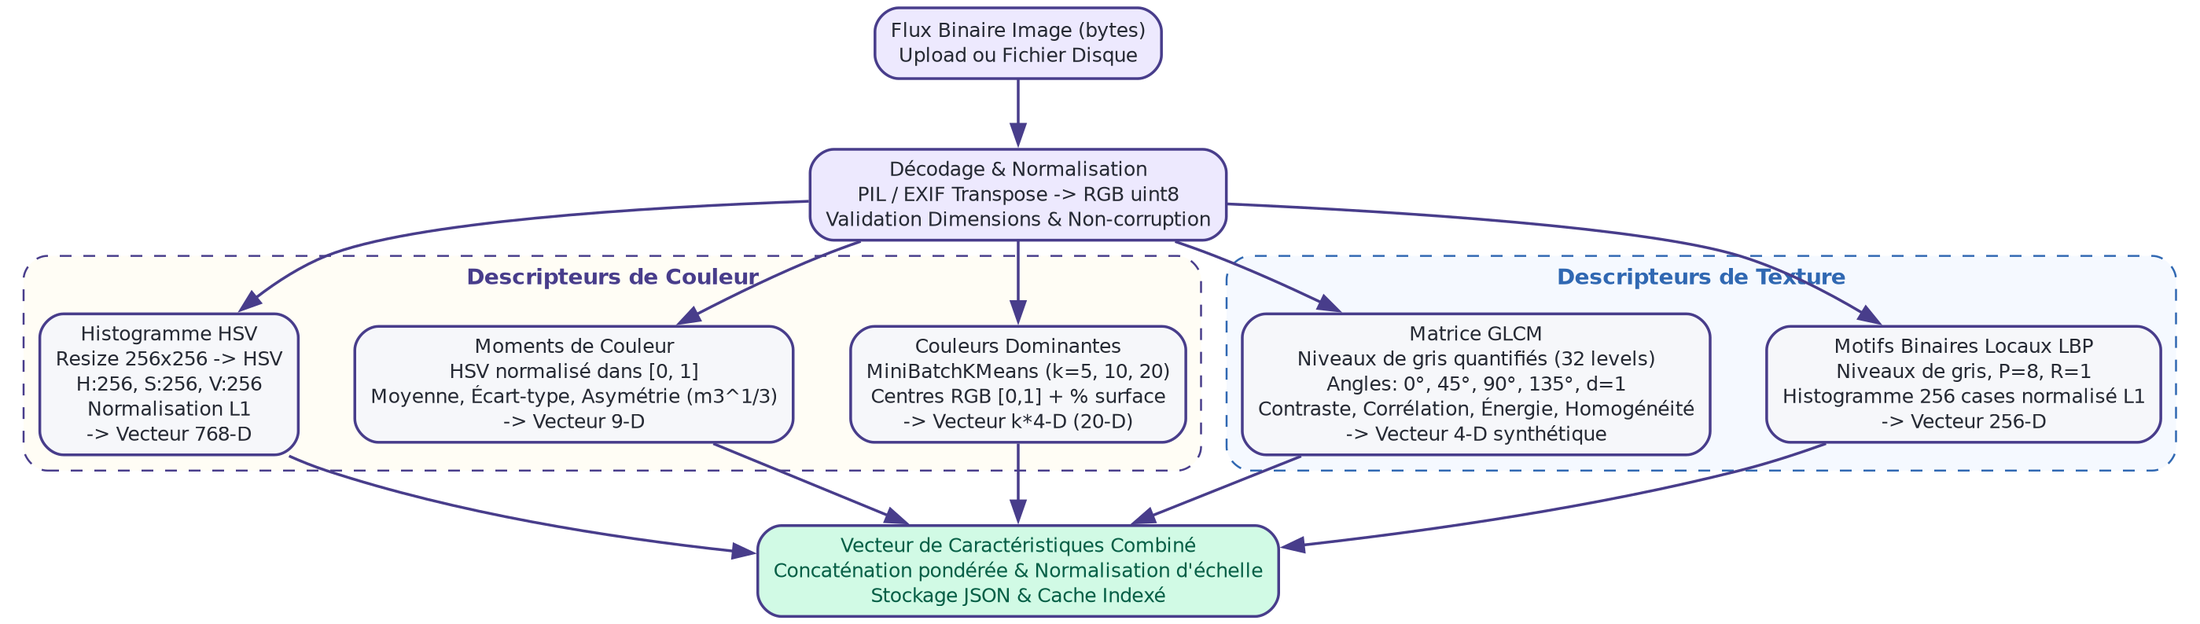
\includegraphics[width=0.78\textwidth]{images/05-pipeline-extraction-descripteurs.png}
\caption{Pipeline d'extraction multi-facettes et construction de la signature visuelle}
\label{fig:pipeline_descripteurs}
\end{figure}

Avant toute opération de filtrage, la méthode statique \texttt{decode\_image\_rgb} procède à un prétraitement unifié~:
\begin{enumerate}
    \item \textbf{Correction d'orientation EXIF~:} Application de \texttt{ImageOps.exif\_transpose} afin que les images issues d'appareils mobiles ou reflex soient redressées dans leur orientation physique réelle sans biais angulaire.
    \item \textbf{Normalisation d'espace colorimétrique~:} Conversion systématique en format RGB non compressé sous forme de tableau NumPy de type \texttt{uint8} à trois canaux de forme $(H, W, 3)$.
    \item \textbf{Contrôle de conformité~:} Rejet immédiat de tout flux vide ou corrompu par la levée de l'exception typée \texttt{InvalidImageStreamError}.
\end{enumerate}

\section{Descripteurs de Couleur}

La couleur traduit la composition spectrale d'une scène. Perceptra combine trois descripteurs complémentaires offrant des niveaux d'abstraction variés.

\subsection{1. Histogramme de Couleur HSV 768-D Normalisé L1}
Bien que le format d'acquisition soit usuellement le RGB, les trois composantes sont hautement corrélées entre elles et sensibles aux variations d'éclairement. Nous procédons donc à une conversion dans l'espace \textbf{HSV} (\textit{Teinte, Saturation, Valeur}).

L'image est d'abord rééchantillonnée en dimensions normalisées $256 \times 256$ pixels par interpolation \texttt{cv2.INTER\_AREA} afin d'uniformiser la complexité algorithmique. Ensuite, les histogrammes individuels pour chaque canal sont calculés via \texttt{cv2.calcHist}~:
\begin{itemize}
    \item Canal $H$ (Teinte) : quantifié sur 256 intervalles dans la plage $[0, 180[$~;
    \item Canal $S$ (Saturation) : quantifié sur 256 intervalles dans la plage $[0, 256[$~;
    \item Canal $V$ (Valeur) : quantifié sur 256 intervalles dans la plage $[0, 256[$.
\end{itemize}

Afin de conférer au descripteur une invariance stricte à l'échelle de l'image, chaque canal subit une \textbf{normalisation $L_1$} indépendante~:
\begin{equation}
\tilde{h}_c(k) = \frac{h_c(k)}{\sum_{i=0}^{255} h_c(i)}, \quad \forall c \in \{H, S, V\}, \quad k \in [0, 255]
\end{equation}

Les trois vecteurs normalisés de 256 dimensions sont concaténés pour former une signature chromatique globale de \textbf{768 dimensions}~:
\begin{equation}
\mathbf{v}_{\text{hist}} = \big[ \tilde{h}_H(0), \dots, \tilde{h}_H(255), \; \tilde{h}_S(0), \dots, \tilde{h}_S(255), \; \tilde{h}_V(0), \dots, \tilde{h}_V(255) \big] \in \mathbb{R}^{768}
\end{equation}

\subsection{2. Moments Statistiques de Couleur 9-D (Stricker \& Orengo)}
Pour obtenir une représentation extrêmement compacte et robuste au bruit haute fréquence, nous calculons les trois premiers moments statistiques de distribution selon le formalisme de Stricker et Orengo~\cite{stricker1995similarity}.

Les canaux HSV sont au préalable normalisés dans l'intervalle continu $[0, 1]$ ($H$ divisé par 179, $S$ et $V$ divisés par 255). Pour chaque canal $c \in \{H, S, V\}$ de $N$ pixels, les moments sont définis par~:
\begin{enumerate}
    \item \textbf{Moyenne $\mu_c$~:} $\mu_c = \frac{1}{N} \sum_{i=1}^{N} p_{c, i}$
    \item \textbf{Écart-type $\sigma_c$~:} $\sigma_c = \sqrt{\frac{1}{N} \sum_{i=1}^{N} (p_{c, i} - \mu_c)^2}$
    \item \textbf{Asymétrie signée $s_c$~:} Pour préserver le signe lors de l'extraction de la racine cubique~:
    \begin{equation}
    m_{3, c} = \frac{1}{N} \sum_{i=1}^{N} (p_{c, i} - \mu_c)^3, \quad s_c = \operatorname{sign}(m_{3, c}) \cdot \sqrt[3]{|m_{3, c}|}
    \end{equation}
\end{enumerate}

Le vecteur résultant compile ces 9 valeurs réelles~:
\begin{equation}
\mathbf{v}_{\text{moments}} = [\mu_H, \sigma_H, s_H, \; \mu_S, \sigma_S, s_S, \; \mu_V, \sigma_V, s_V] \in \mathbb{R}^9
\end{equation}

\subsection{3. Couleurs Dominantes par Partitionnement MiniBatchKMeans}
L'algorithme \texttt{MiniBatchKMeans} est appliqué sur l'image sous-échantillonnée ($128 \times 128$) avec $k=5$ centroïdes RGB et une graine aléatoire fixe (\texttt{random\_state=42}). Pour chaque centroïde $j \in [1, 5]$ ordonné par poids volumique $w_j \in [0, 1]$, la composante vectorielle compile les couleurs normalisées et la surface~:
\begin{equation}
\mathbf{c}_j = \left[ \frac{\bar{R}_j}{255}, \; \frac{\bar{G}_j}{255}, \; \frac{\bar{B}_j}{255}, \; w_j \right] \implies \mathbf{v}_{\text{dom}} \in \mathbb{R}^{20}
\end{equation}

\section{Descripteurs de Texture}

\subsection{1. Matrice de Co-occurrence de Niveaux de Gris (GLCM)}
L'image en niveaux de gris est quantifiée linéairement sur $L=32$ niveaux d'intensité. Pour une distance $d=1$ selon les quatre angles $\theta \in \{0^\circ, 45^\circ, 90^\circ, 135^\circ\}$, les quatre métriques de Haralick et al.~\cite{haralick1973textural} sont évaluées~:
\begin{align}
\text{Contraste~:} \quad & f_{\text{con}}(\theta) = \sum_{i=0}^{L-1}\sum_{j=0}^{L-1} (i - j)^2 P_{\theta}(i, j) \\
\text{Corrélation~:} \quad & f_{\text{corr}}(\theta) = \sum_{i=0}^{L-1}\sum_{j=0}^{L-1} \frac{(i - \mu_i)(j - \mu_j) P_{\theta}(i, j)}{\sigma_i \sigma_j} \\
\text{Énergie (ASM)~:} \quad & f_{\text{ene}}(\theta) = \sum_{i=0}^{L-1}\sum_{j=0}^{L-1} P_{\theta}(i, j)^2 \\
\text{Homogénéité~:} \quad & f_{\text{hom}}(\theta) = \sum_{i=0}^{L-1}\sum_{j=0}^{L-1} \frac{P_{\theta}(i, j)}{1 + (i - j)^2}
\end{align}

Le vecteur synthétique $\mathbf{v}_{\text{glcm}} \in \mathbb{R}^4$ compile ces quatre grandeurs moyennées sur les 4 orientations, conférant une invariance stricte aux rotations planes.

\subsection{2. Motifs Binaires Locaux (LBP -- Local Binary Patterns)}
Pour chaque pixel central $g_c$, nous considérons ses $P=8$ voisins équidistants à rayon $R=1$~:
\begin{equation}
LBP_{P, R}(x_c, y_c) = \sum_{p=0}^{P-1} s(g_p - g_c) \cdot 2^p, \quad \text{où } s(z) = \begin{cases} 1 & \text{si } z \ge 0 \\ 0 & \text{si } z < 0 \end{cases}
\end{equation}
L'histogramme des 256 occurrences est normalisé par la somme totale ($L_1$), produisant $\mathbf{v}_{\text{lbp}} \in \mathbb{R}^{256}$.

\begin{table}[H]
\centering
\rowcolors{2}{LightGray}{white}
\begin{tabularx}{\textwidth}{>{\bfseries}p{3.5cm}p{1.8cm}p{2.5cm}X}
\toprule
\rowcolor{TableHeader}
\color{white}Nom du Descripteur & \color{white}Dim. & \color{white}Espace / Entrée & \color{white}Propriétés Clés \\
\midrule
\texttt{color\_histogram} & 768 & HSV ($256 \times 3$) & Normalisation L1 par canal, robuste aux variations lumineuses. \\
\texttt{color\_moments} & 9 & HSV norm. $[0, 1]$ & Moyenne, écart-type et asymétrie signée $\sqrt[3]{m_3}$ ; très compact. \\
\texttt{dominant\_colors} & 20 & RGB ($k=5$) & 5 centroïdes RGB ordonnés par importance avec pourcentages surfaciques. \\
\texttt{glcm} & 4 & Niveaux de gris (32) & Contraste, corrélation, énergie et homogénéité moyennés sur 4 angles. \\
\texttt{lbp\_histogram} & 256 & Niveaux de gris & Voisinage $P=8, R=1$, histogramme L1 décrivant la micro-texture locale. \\
\bottomrule
\end{tabularx}
\caption{Synthèse dimensionnelle et caractéristiques des descripteurs de Perceptra}
\label{tab:descripteurs_synthese}
\end{table}

\chapter{Moteur de Similarité et Recherche par l'Image}
\label{chap:recherche}

\section{Espaces Métriques et Mesures de Proximité}

La recherche par le contenu nécessite de projeter les images au sein d'un espace vectoriel normé et d'évaluer leur proximité relative. Cette fonction est assurée par le composant \texttt{SimilarityEngine} (\texttt{src/services/similarity\_engine.py}).

Soit $\mathbf{q} \in \mathbb{R}^D$ le vecteur représentant la requête visuelle de l'utilisateur et $\mathbf{c} \in \mathbb{R}^D$ le vecteur correspondant à une image candidate issue de la collection indexée.

Toutes les mesures de proximité dans Perceptra sont calibrées pour appartenir strictement à l'intervalle $[0, 1]$, où la valeur $1.0$ indique une identité visuelle parfaite et $0.0$ une divergence totale.

\begin{infobox}{Métrique Cosinus Normalisée (Défaut)}
La similarité cosinus mesure l'angle géométrique entre deux vecteurs indépendamment de leur magnitude globale, ce qui s'avère particulièrement pertinent pour comparer des histogrammes de fréquences ou de textures~:
\begin{equation}
\cos(\mathbf{q}, \mathbf{c}) = \frac{\mathbf{q} \cdot \mathbf{c}}{\|\mathbf{q}\|_2 \cdot \|\mathbf{c}\|_2} \implies S_{\text{cos}}(\mathbf{q}, \mathbf{c}) = \frac{1 + \cos(\mathbf{q}, \mathbf{c})}{2} \in [0, 1]
\end{equation}
Les évaluations expérimentales sur GHIM-10K confirment la supériorité systématique de la similarité cosinus, surpassant la distance euclidienne de plus de 10 points de précision ($P@5 = 52,5\,\%$ contre $42,0\,\%$).
\end{infobox}

\begin{infobox}{Métrique Euclidienne Inversée}
Lorsque l'utilisateur sélectionne la métrique euclidienne $L_2$, la distance géométrique $d_2(\mathbf{q}, \mathbf{c}) = \|\mathbf{q} - \mathbf{c}\|_2$ est convertie en score de similarité borné selon la décroissance harmonique standard~:
\begin{equation}
S_{\text{euc}}(\mathbf{q}, \mathbf{c}) = \frac{1}{1 + \|\mathbf{q} - \mathbf{c}\|_2} \in [0, 1]
\end{equation}
\end{infobox}

\section{Agrégation Convexe Multi-Descripteurs}

Pour éviter l'écueil classique de la «~malédiction de la dimensionnalité~» induit par la concaténation brute d'espaces hétérogènes, Perceptra maintient chaque descripteur dans son sous-espace métrique propre.

Soit $\mathcal{F}$ l'ensemble des familles de descripteurs actives. Pour chaque descripteur $j \in \mathcal{F}$, nous disposons d'un vecteur de requête $\mathbf{q}_j$, d'un candidat $\mathbf{c}_j$ et d'un poids $w_j \ge 0$. Les poids actifs sont préalablement normalisés sous contrainte convexe~:
\begin{equation}
\tilde{w}_j = \frac{w_j}{\sum_{k \in \mathcal{F}} w_k}, \quad \text{tel que } \sum_{j \in \mathcal{F}} \tilde{w}_j = 1.0
\end{equation}

La similarité globale $S(\mathbf{q}, \mathbf{c})$ entre l'image requête et l'image candidate est alors formulée comme la combinaison linéaire convexe des similarités individuelles~:
\begin{equation}
S(\mathbf{q}, \mathbf{c}) = \sum_{j \in \mathcal{F}} \tilde{w}_j \cdot S_j(\mathbf{q}_j, \mathbf{c}_j)
\end{equation}

\section{Décomposition Analytique et Ordonnancement Top-K}

Pour offrir une transparence maximale à l'utilisateur, la méthode \texttt{aggregate\_multi\_feature\_similarity} extrait simultanément la décomposition des affinités par famille conceptuelle~:
\begin{itemize}
    \item \textbf{Similarité Chromatique ($S_{\text{color}}$)~:} Moyenne arithmétique des scores des composantes de couleur actives (\texttt{color\_histogram}, \texttt{color\_moments}, \texttt{dominant\_colors})~;
    \item \textbf{Similarité Texturale ($S_{\text{texture}}$)~:} Moyenne arithmétique des scores des composantes texturales actives (\texttt{glcm}, \texttt{lbp\_histogram})~;
    \item \textbf{Scores fins par descripteur~:} Dictionnaire associatif $\{j: S_j(\mathbf{q}_j, \mathbf{c}_j)\}$.
\end{itemize}

Le service de requête \texttt{QueryService} (\texttt{src/services/query\_service.py}) orchestre l'exécution de la recherche en mémoire~: filtrage du périmètre (\texttt{all}, \texttt{ghim10k}, \texttt{my\_images}), balayage matriciel vectorisé sous NumPy évaluant 10\,000 vecteurs en moins de 45 millisecondes, tri décroissant et extraction des $K$ meilleurs résultats (\texttt{Top-K}).

\chapter{Estimation de la Pertinence des Descripteurs (FRE)}
\label{chap:fre}

\section{Introduction et Mission du Groupe 13}

Au sein de l'architecture de Perceptra, le module \textbf{Feature Relevance Estimation (FRE)} constitue la contribution scientifique et algorithmique assignée de manière exclusive au \textbf{Groupe 13}.

Les systèmes CBIR classiques considèrent invariablement que tous les descripteurs visuels possèdent un pouvoir discriminant équivalent. Or, l'intention de l'utilisateur est fondamentalement contextuelle~: lors de la recherche de couchers de soleil, la teinte globale et la saturation sont déterminantes, tandis que pour des textures régulières (tissus, façades), le GLCM et le LBP sont prépondérants.

L'algorithme \textbf{FRE} formalise mathématiquement cette intuition~: il observe les images annotées par l'utilisateur (pertinentes ou rejetées), quantifie la pertinence relative de chaque descripteur à partir de sa variance et de son pouvoir séparateur, et reconfigure automatiquement l'espace métrique pour les itérations suivantes.

\begin{figure}[H]
\centering
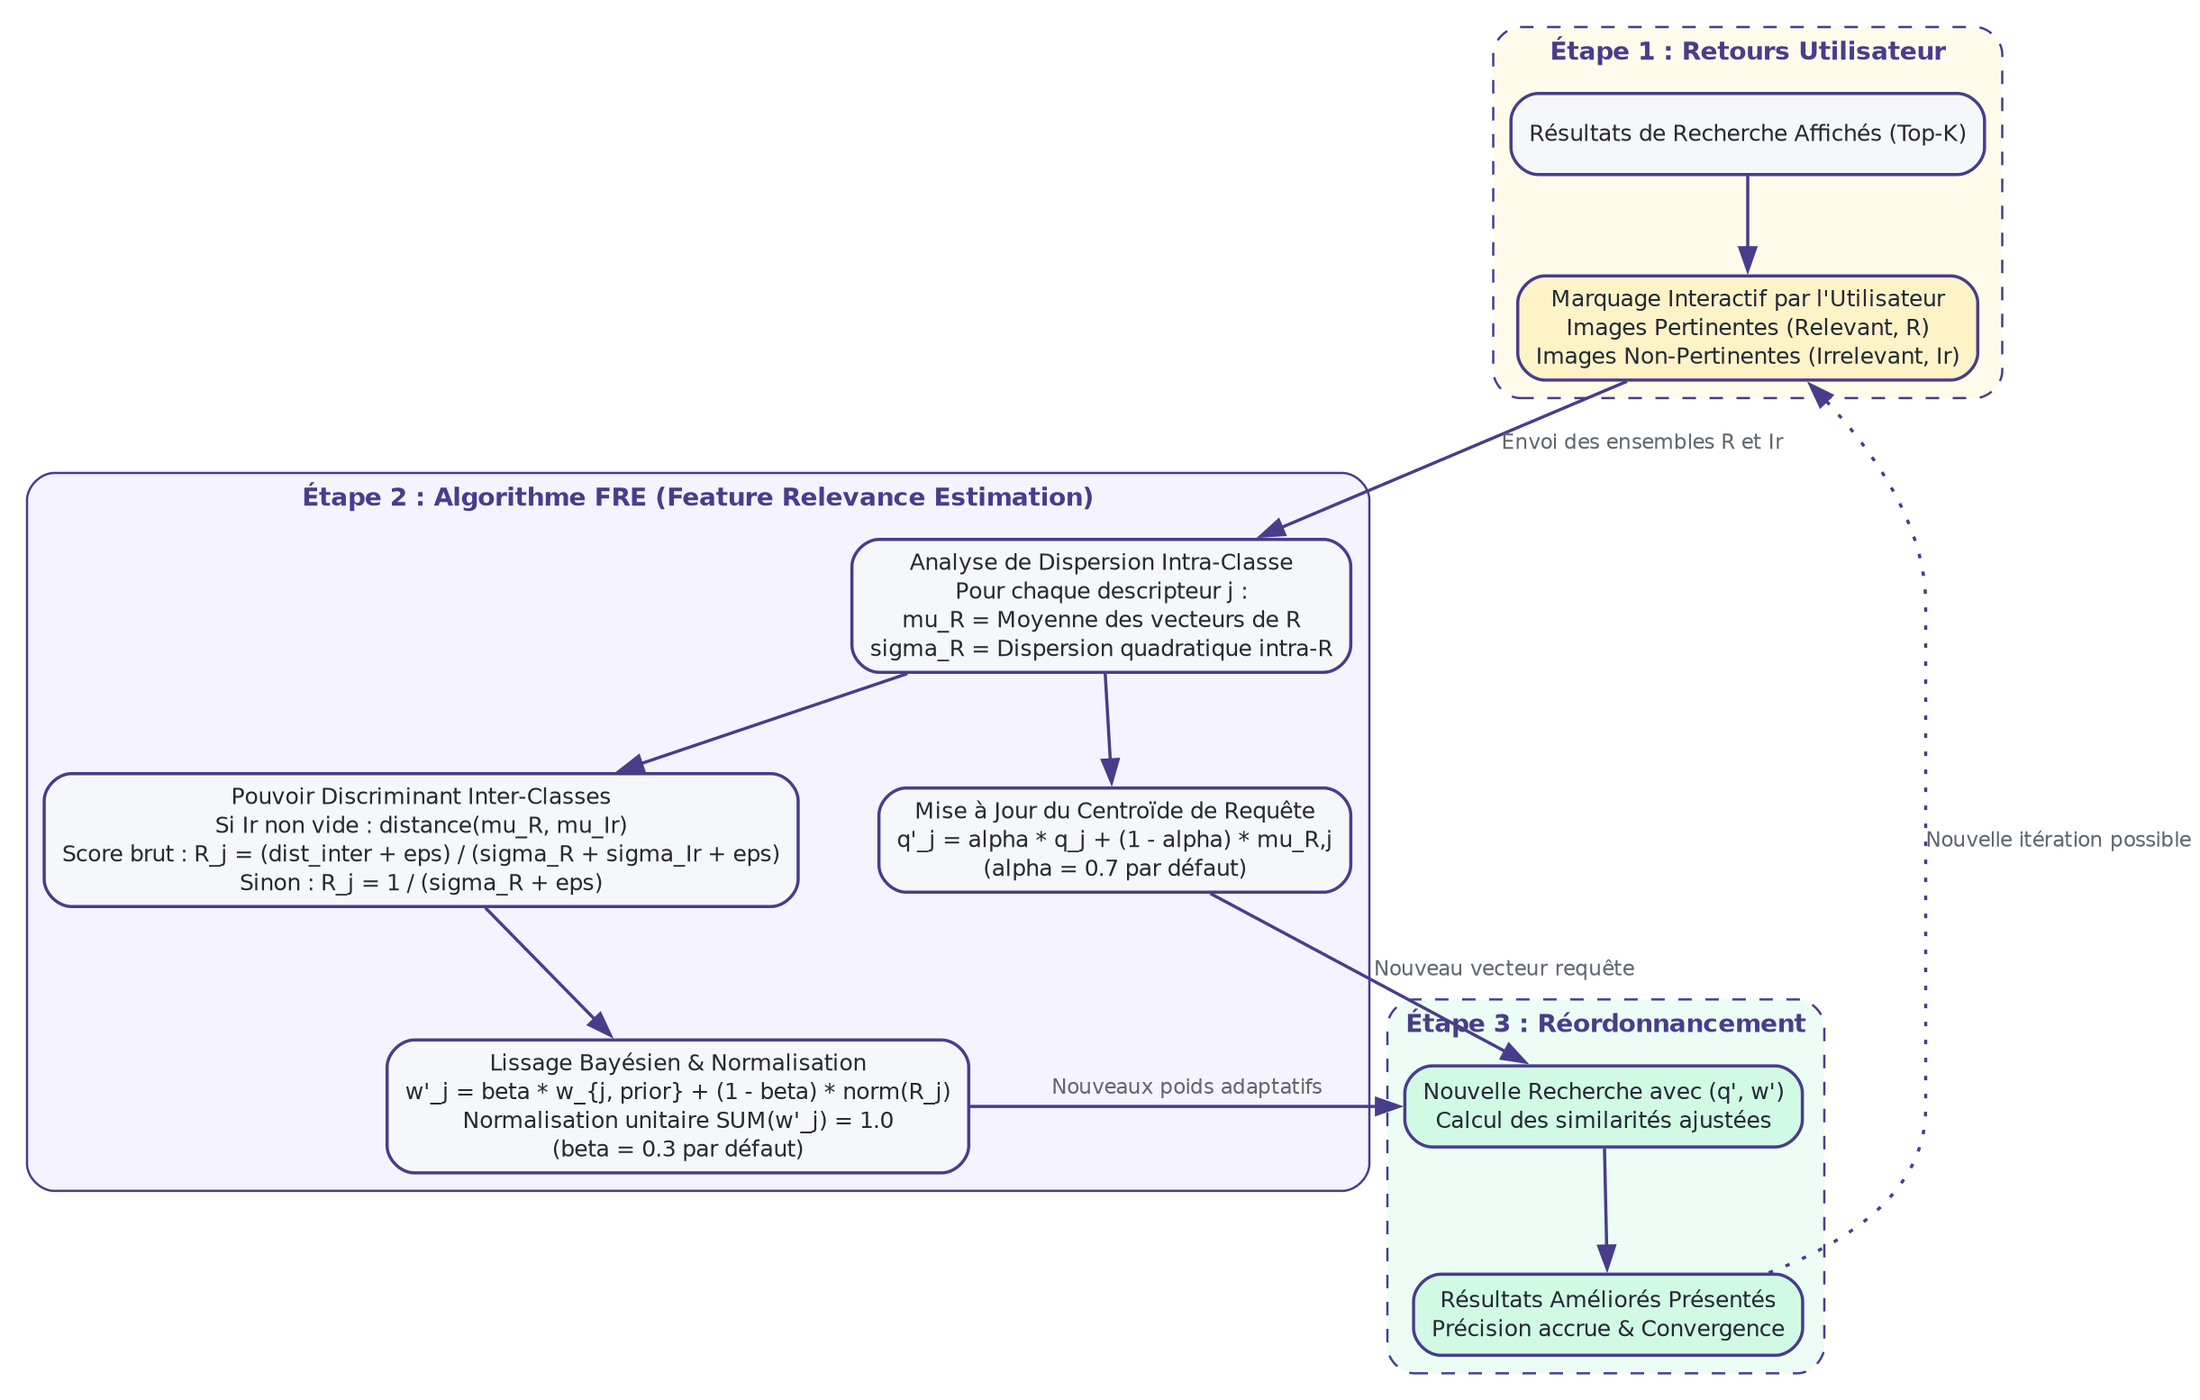
\includegraphics[width=0.66\textwidth]{images/07-boucle-relevance-feedback-fre.png}
\caption{Boucle de rétroaction adaptative FRE (Feature Relevance Estimation)}
\label{fig:boucle_fre}
\end{figure}

\section{Formulation Mathématique de l'Algorithme FRE}

Soit un espace de recherche caractérisé par un ensemble de familles de descripteurs $\mathcal{F}$. L'utilisateur labellise les résultats affichés en deux ensembles disjoints~:
\begin{itemize}
    \item L'ensemble des images pertinentes~: $\mathcal{R} = \{\mathbf{x}_1^{(r)}, \dots, \mathbf{x}_{N_r}^{(r)}\}$, avec $N_r \ge 1$~;
    \item L'ensemble des images non-pertinentes~: $\mathcal{I} = \{\mathbf{x}_1^{(i)}, \dots, \mathbf{x}_{N_i}^{(i)}\}$, avec $N_i \ge 0$.
\end{itemize}

L'algorithme se déroule en quatre étapes canoniques~:

\subsection{Étape 1 : Centroïde et Dispersion Intra-Classe}
Le centroïde de pertinence $\boldsymbol{\mu}_{R, j}$ est la moyenne arithmétique des vecteurs d'exemples positifs pour le descripteur $j$~:
\begin{equation}
\boldsymbol{\mu}_{R, j} = \frac{1}{N_r} \sum_{k=1}^{N_r} \mathbf{x}_{k, j}^{(r)}
\end{equation}

La compacité intra-classe $\sigma_{R, j}$ mesure la cohérence des exemples pertinents pour le descripteur $j$~:
\begin{equation}
\sigma_{R, j} = \begin{cases}
\sqrt{ \frac{1}{N_r} \sum_{k=1}^{N_r} \|\mathbf{x}_{k, j}^{(r)} - \boldsymbol{\mu}_{R, j}\|_2^2 } & \text{si } N_r > 1 \\
\|\mathbf{x}_{1, j}^{(r)} - \mathbf{q}_j\|_2 & \text{si } N_r = 1
\end{cases}
\end{equation}
Une faible valeur de $\sigma_{R, j}$ démontre que les exemples positifs partagent une signature quasi-identique pour le descripteur $j$, signalant une caractéristique invariante essentielle.

\subsection{Étape 2 : Séparabilité Inter-Classes (Critère de Fisher)}
Si des exemples négatifs sont fournis ($N_i \ge 1$), nous calculons leur centroïde $\boldsymbol{\mu}_{I, j}$ et leur dispersion $\sigma_{I, j}$. La distance inter-classes s'exprime par $d_{\text{inter}, j} = \|\boldsymbol{\mu}_{R, j} - \boldsymbol{\mu}_{I, j}\|_2$.

Le score brut de pertinence $R_j$ s'inspire du discriminant linéaire de Fisher (ratio entre dispersion inter et intra-classe)~:
\begin{equation}
R_j = \begin{cases}
\frac{d_{\text{inter}, j} + \epsilon}{\sigma_{R, j} + \sigma_{I, j} + \epsilon} & \text{si } N_i \ge 1 \\
\frac{1}{\sigma_{R, j} + \epsilon} & \text{si } N_i = 0
\end{cases}
\end{equation}
où $\epsilon = 10^{-4}$ prévient toute division par zéro.

\subsection{Étape 3 : Lissage Bayésien et Normalisation des Poids}
Les scores bruts sont normalisés sous contrainte unitaire $\tilde{R}_j = R_j / \sum_{k \in \mathcal{F}} R_k$. Afin d'éviter les sur-ajustements (\textit{overfitting}) lors des premiers retours, un paramètre de lissage avec mémoire d'inertie $\beta \in [0, 1]$ (fixé à $\beta = 0.3$) combine les poids a priori avec la nouvelle estimation~:
\begin{equation}
w'_j = \beta \cdot w_{j, \text{prior}} + (1 - \beta) \cdot \tilde{R}_j \implies w_{j, \text{final}} = \frac{w'_j}{\sum_{k \in \mathcal{F}} w'_k}
\end{equation}

\subsection{Étape 4 : Déplacement Guidé du Centroïde de Requête}
Parallèlement à l'ajustement des poids, le vecteur de requête $\mathbf{q}_j$ est translaté vers le barycentre des exemples positifs via un coefficient de momentum $\alpha = 0.7$~:
\begin{equation}
\mathbf{q}'_j = \alpha \cdot \mathbf{q}_j + (1 - \alpha) \cdot \boldsymbol{\mu}_{R, j}
\end{equation}

\section{Implémentation Logicielle et Diagnostics}

L'implémentation de ce modèle dans la classe \texttt{FeatureRelevanceEstimator} (\texttt{src/services/relevance\_feedback.py}) garantit une convergence rapide et une stabilité numérique totale.

\begin{lstlisting}[language=Python, caption={Extrait central de l'algorithme FRE (src/services/relevance\_feedback.py)}]
# Critere de type Fisher : ecart inter-classe / dispersion intra-classe
if irr_vecs:
    irr_mat = np.vstack(irr_vecs)
    mu_irr = np.mean(irr_mat, axis=0)
    between_distance = float(np.linalg.norm(mu_r - mu_irr))
    dispersion_irr = np.sqrt(max(0.0, float(np.mean(np.sum((irr_mat - mu_irr)**2, axis=1)))))
    relevance_val = (between_distance + cls.EPSILON) / (dispersion_r + dispersion_irr + cls.EPSILON)
else:
    between_distance = 0.0
    relevance_val = 1.0 / (dispersion_r + cls.EPSILON)

# Deplacement du centroide de requete
refined_q = alpha_query * q_vec + (1.0 - alpha_query) * mu_r

# Lissage avec la configuration a priori
blended = beta_prior * prior_w + (1.0 - beta_prior) * norm_estimated[ft]
\end{lstlisting}

\chapter{Frontend et Expérience Utilisateur}
\label{chap:frontend}

\section{Architecture Frontend et Paradigme Svelte 5 Runes}

L'application web de Perceptra (\texttt{web/}) repose sur une stack front-end d'avant-garde combinant \textbf{SvelteKit 3} et le moteur de réactivité unifié \textbf{Svelte 5}. Contrairement aux frameworks historiques basés sur un DOM virtuel lourd (Virtual DOM comme React ou Vue), Svelte compile les composants en instructions JavaScript chirurgicales directes, offrant des performances d'affichage optimales indispensables pour manipuler des collections de milliers d'images.

\begin{figure}[H]
\centering
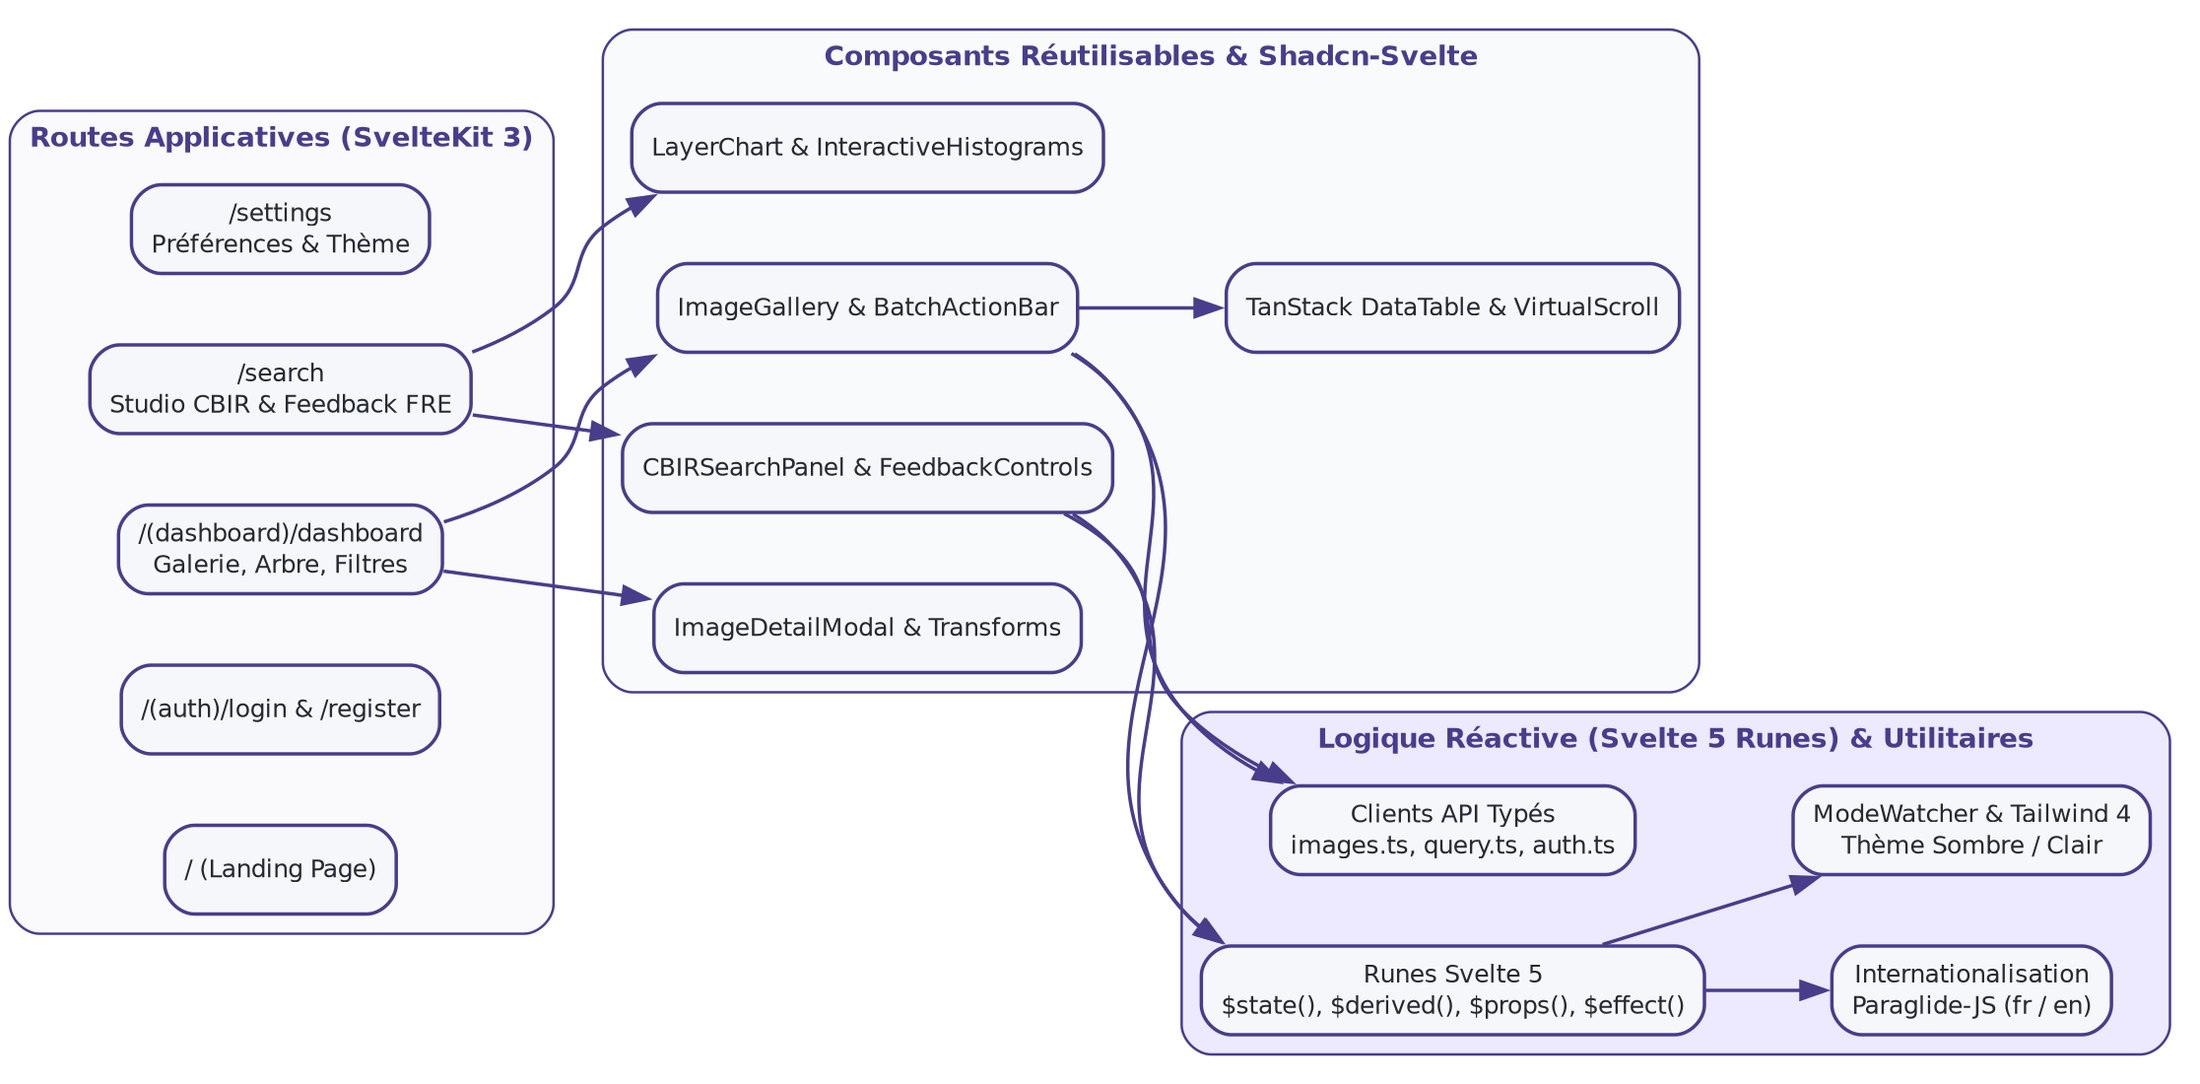
\includegraphics[width=0.78\textwidth]{images/08-architecture-frontend-sveltekit.png}
\caption{Architecture réactive du frontend SvelteKit et organisation des composants}
\label{fig:frontend_arch}
\end{figure}

Le développement exploite exhaustivement les \textbf{Runes} introduites par Svelte~5~:
\begin{itemize}
    \item \texttt{\$state()} : Déclaration explicite des variables d'état réactives (ex: images sélectionnées, filtres actifs, résultats)~;
    \item \texttt{\$derived()} : Calcul automatisé et mémorisé de propriétés dérivées (ex: comptage filtré, somme des poids)~;
    \item \texttt{\$props()} : Déclaration strictement typée des propriétés transmises aux composants enfants via TypeScript~;
    \item \texttt{\$effect()} : Gestion déterministe des effets de bord (synchronisation API, persistance du thème).
\end{itemize}

\section{Système de Conception : Shadcn-Svelte et Tailwind CSS 4}

Pour garantir une identité visuelle professionnelle et accessible, Perceptra intègre la suite de composants \textbf{Shadcn-Svelte} articulée sur les primitives accessibles de \textbf{Bits UI} et stylisée avec le moteur \textbf{Tailwind CSS 4}~:
\begin{itemize}
    \item \textbf{Thématisation Dynamique~:} Prise en charge native du mode sombre et mode clair pilotée par \texttt{mode-watcher}, avec respect strict des contrastes WCAG AAA.
    \item \textbf{Composants Fondamentaux~:} Modales de dialogue (\texttt{Dialog}), volets latéraux contextuels (\texttt{Sheet}), tiroirs coulissants tactiles (\texttt{Drawer} via Vaul-Svelte), menus déroulants et notifications toast instantanées (\texttt{svelte-sonner}).
    \item \textbf{Tableaux de Données Avancés~:} Intégration de \texttt{@tanstack/svelte-table} pour le tri multi-colonnes, la recherche textuelle en temps réel et la pagination virtuelle.
\end{itemize}

\section{Modules Applicatifs et Écrans Principaux}

L'interface de Perceptra s'articule autour de trois espaces majeurs~:

\subsection{1. Galerie de Médias et Organisation (\texttt{/dashboard})}
\begin{itemize}
    \item \textbf{Explorateur Arborescent de Catégories~:} Panneau latéral rétractable affichant l'arbre hiérarchique des dossiers créés par l'utilisateur avec comptage réactif des médias rattachés.
    \item \textbf{Grille Réactive d'Images~:} Affichage adaptatif avec chargement paresseux (\textit{lazy loading}) des vignettes optimisées et statut favori.
    \item \textbf{Barre d'Actions par Lot (\texttt{BatchActionBar})~:} Barre d'action flottante surgissant lors de la sélection multiple pour autoriser la suppression groupée ou l'exportation.
\end{itemize}

\subsection{2. Modale de Retouche et Caractérisation (\texttt{ImageDetailModal})}
Visualiseur exhaustif des caractéristiques physiques et atelier complet de transformation non destructive~: recadrage avec règle des tiers, curseurs de redimensionnement proportionnel et rotations libres.

\subsection{3. Studio de Recherche CBIR et Rétroaction (\texttt{/search})}
\begin{enumerate}
    \item \textbf{Dépôt de la Requête Visuelle~:} Glisser-déposer d'une image locale ou sélection dans la galerie.
    \item \textbf{Panneau de Configuration des Poids~:} Curseurs ergonomiques pour doser l'influence relative de chaque descripteur.
    \item \textbf{Grille de Résultats Ordonnés~:} Restitution instantanée des $K$ images les plus proches avec badges de similarité globale, chromatique et texturale.
    \item \textbf{Contrôles de Pertinence et FRE~:} Bouton vert (Pertinent) et bouton rouge (Non-pertinent). Le bouton «~Réestimer la pertinence (FRE)~» déclenche l'ajustement adaptatif et le réordonnancement de la collection.
\end{enumerate}

\section{Visualisations Analytiques et Internationalisation Bilingue}

Perceptra intègre la bibliothèque \textbf{LayerChart} et \textbf{D3.js} pour restituer les histogrammes spectro-chromatiques sous forme de barres SVG colorées et tracer l'évolution des poids FRE. L'internationalisation est assurée par \textbf{Paraglide-JS}, garantissant un bilinguisme intégral (Français/Anglais) compilé statiquement avec vérification TypeScript à zéro surcharge d'exécution.

\chapter{Gestion des Données et Stratégie de Stockage}
\label{chap:donnees}

\section{Modélisation Relationnelle de la Base de Données}

La persistance des métadonnées et la structuration des sessions de recherche reposent sur un modèle relationnel strict conçu sous \textbf{SQLAlchemy 2.0}. Le modèle relationnel de Perceptra assure une intégrité référentielle absolue, renforcée par des contraintes d'unicité et des suppressions en cascade (\texttt{CASCADE ON DELETE}).

\begin{figure}[htbp]
\centering
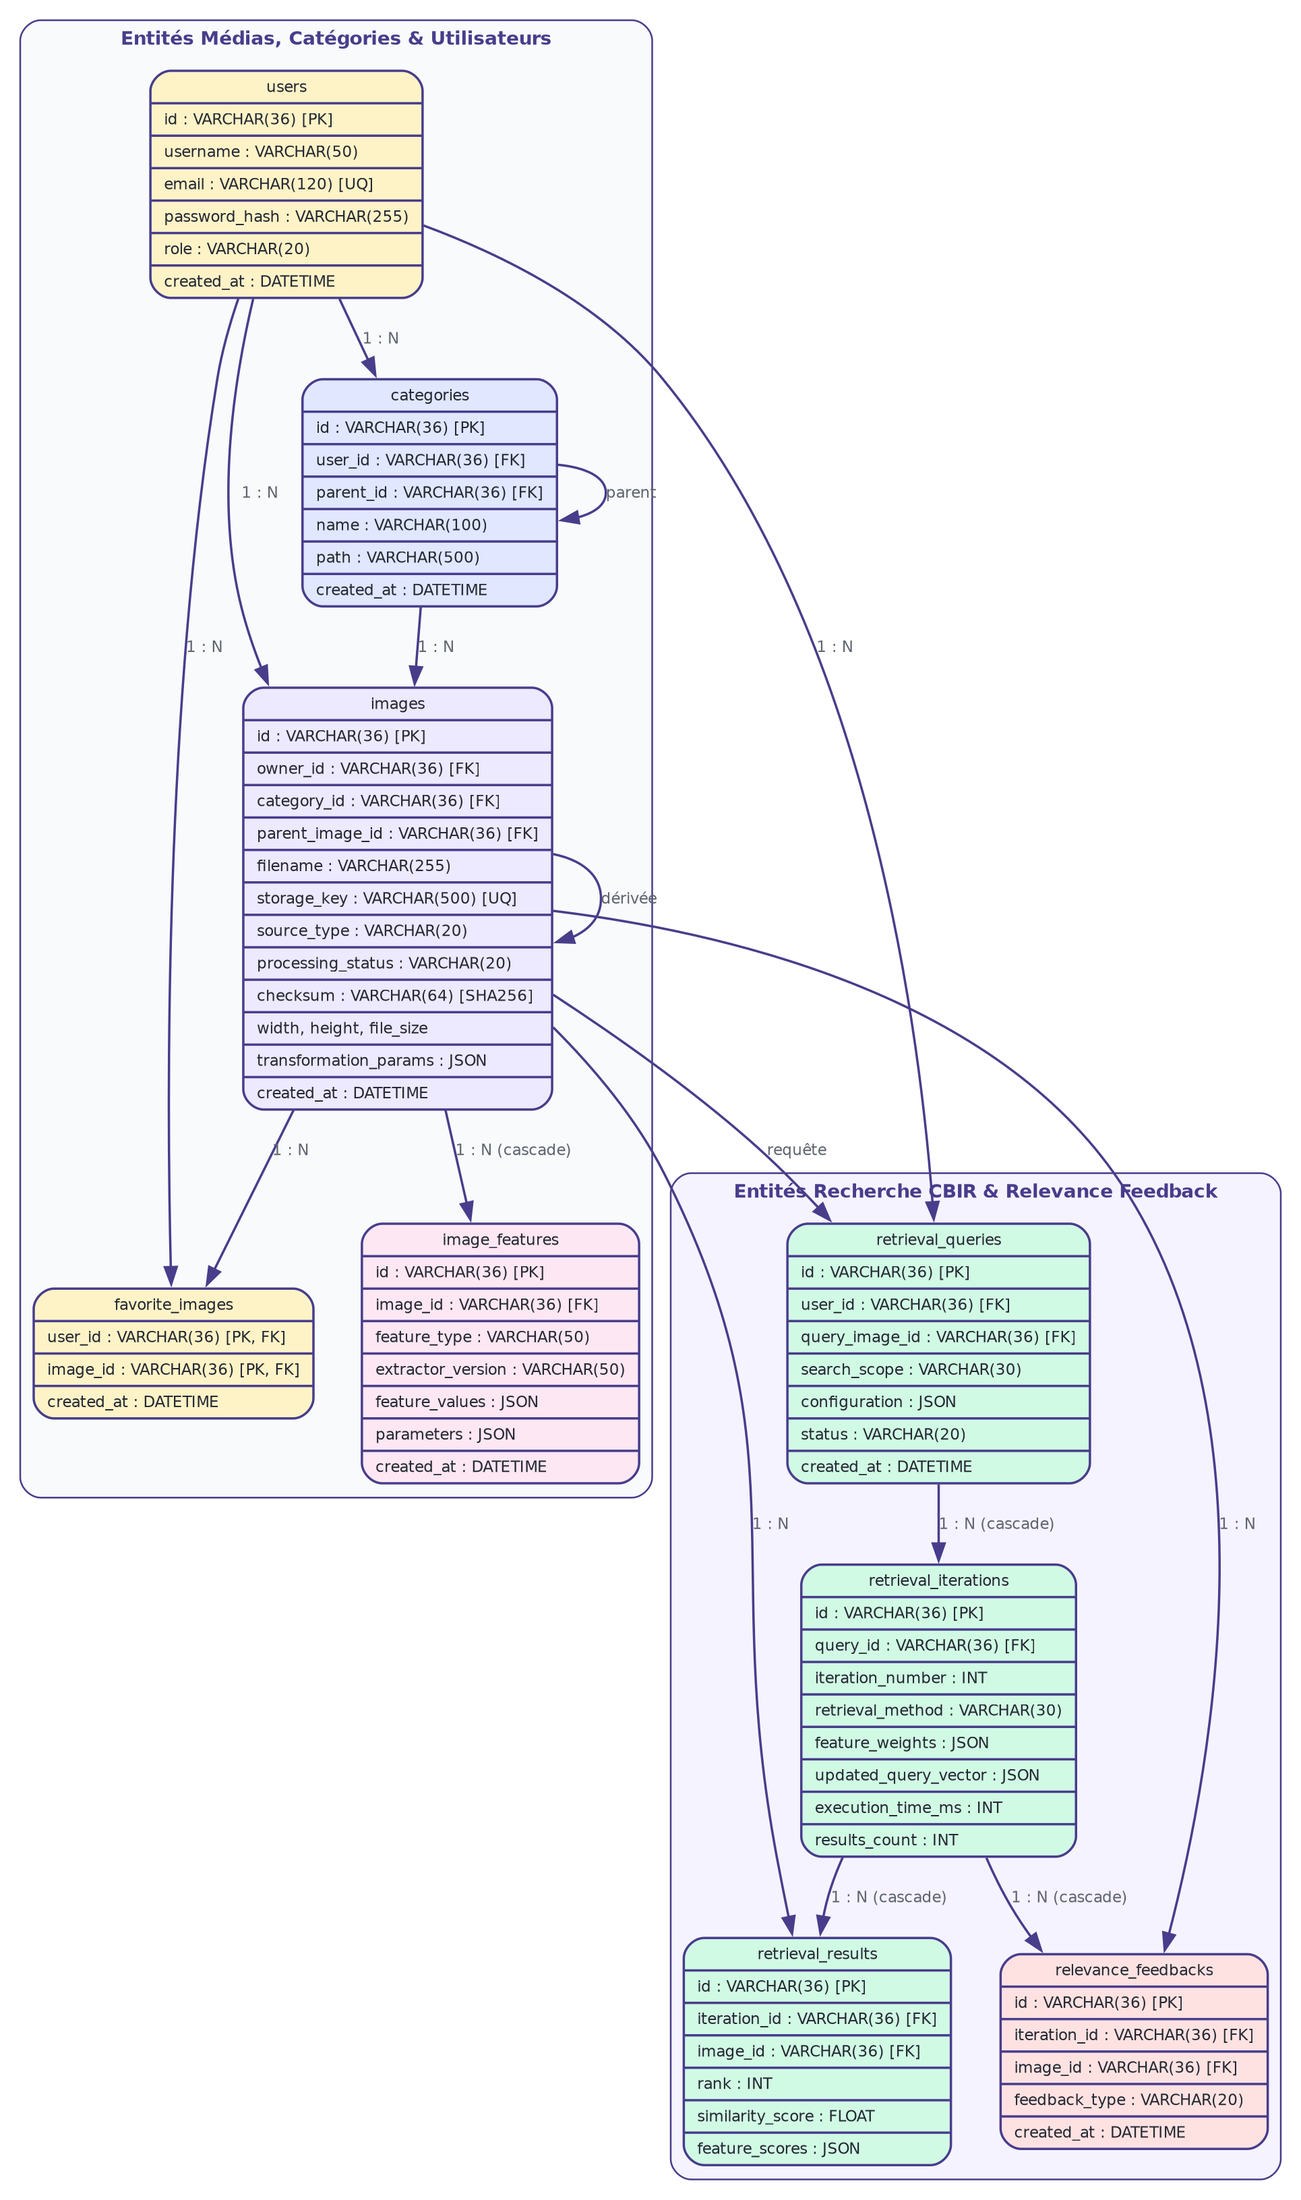
\includegraphics[width=0.48\textwidth]{images/09-schema-relationnel-db.png}
\caption{Schéma Entité-Association complet de la base de données de Perceptra}
\label{fig:schema_db}
\end{figure}

Le tableau~\ref{tab:entites_db} synthétise le rôle et les contraintes des entités principales du schéma.

\begin{table}[H]
\centering
\rowcolors{2}{LightGray}{white}
\begin{tabularx}{\textwidth}{>{\bfseries}p{3.2cm}p{3.0cm}X}
\toprule
\rowcolor{TableHeader}
\color{white}Table & \color{white}Clé Primaire & \color{white}Rôle et Contraintes Notables \\
\midrule
\texttt{users} & \texttt{id (UUID-36)} & Comptes utilisateurs, mot de passe haché par PBKDF2-HMAC-SHA256, rôle (\texttt{admin}, \texttt{user}). \\
\texttt{categories} & \texttt{id (UUID-36)} & Organisation arborescente, clé étrangère réflexive \texttt{parent\_id} pour la hiérarchie parent-enfant, chemin calculé \texttt{path}. \\
\texttt{images} & \texttt{id (UUID-36)} & Métadonnées physiques, clé de stockage unique \texttt{storage\_key}, condensat \texttt{checksum} (SHA-256 indexé), dimensions, source (\texttt{dataset}, \texttt{upload}, \texttt{derived}). \\
\texttt{image\_features} & \texttt{id (UUID-36)} & Vecteurs de descripteurs JSON. Contrainte d'unicité stricte \texttt{uq\_image\_feature\_type\_version} sur \texttt{(image\_id, feature\_type, extractor\_version)}. \\
\texttt{retrieval\_queries} & \texttt{id (UUID-36)} & Sessions de recherche initialisées par l'utilisateur, traçabilité du périmètre (\texttt{search\_scope}) et statut. \\
\texttt{retrieval\_iterations} & \texttt{id (UUID-36)} & Itérations successives au sein d'une session, numéro ordonné, méthode de recherche (\texttt{initial}, \texttt{fre}), poids de caractéristiques appliqués, temps en ms. \\
\texttt{retrieval\_results} & \texttt{id (UUID-36)} & Classement des $K$ résultats par itération, rang d'ordonnancement, score global et décomposition par descripteur. \\
\texttt{relevance\_feedbacks} & \texttt{id (UUID-36)} & Annotations interactives de l'utilisateur sur une itération donnée (\texttt{relevant}, \texttt{irrelevant}), horodatées. \\
\bottomrule
\end{tabularx}
\caption{Spécification fonctionnelle des entités de la base de données}
\label{tab:entites_db}
\end{table}

\section{Stratégie de Stockage Hybride et Intégrité Binaire}

Perceptra refuse le stockage direct des flux binaires dans la base de données (colonnes \textit{BLOB}), qui dégrade les tampons mémoire. Le système met en œuvre une \textbf{architecture de stockage hybride}~:
\begin{enumerate}
    \item \textbf{Plan de Données (Système de Fichiers)~:} Les fichiers images bruts sont enregistrés directement sur le volume physique sous des clés UUID4 horodatées (\texttt{storage/uploads/YYYY/MM/<uuid>.<ext>}).
    \item \textbf{Plan de Contrôle (Base SQL)~:} La base de données ne stocke que le descripteur d'accès logique (\texttt{storage\_key}), l'empreinte cryptographique SHA-256, les dimensions et les signatures vectorielles.
    \item \textbf{Vérification d'Intégrité SHA-256~:} Chaque téléversement donne lieu au calcul de son condensat SHA-256. L'index de la colonne \texttt{checksum} détecte instantanément les doublons stricts, économisant l'espace disque et le temps de calcul.
\end{enumerate}

\section{Ingestion du Dataset GHIM-10K et Migrations}

Le jeu de données de référence \textbf{GHIM-10K}~\cite{kaggle_ghim10k} rassemble \textbf{10\,000 images} photographiques réparties en 20 classes thématiques de 500 images chacune (avions, navires, automobiles, feux d'artifice, fleurs, chevaux, montagnes, etc.).

Le service \texttt{DatasetService} (\texttt{src/services/dataset\_service.py}) ingère et pré-indexe cette volumétrie par blocs transactionnels de 500 enregistrements (\texttt{db.session.bulk\_save\_objects}). L'opération s'exécute en environ 18 minutes sur un processeur multi-c\oe{}urs standard, pour un volume de base de données final inférieur à 65 mégaoctets. Les modifications de schéma sont rigoureusement versionnées et appliquées via \textbf{Flask-Migrate} / Alembic.

\chapter{Déploiement, Opérations et Sécurité}
\label{chap:deploiement}

\section{Stratégie de Conteneurisation Multi-Étapes (Docker)}

Pour assurer une portabilité totale du système et éliminer les disparités d'environnements, Perceptra est entièrement conteneurisé à l'aide d'un fichier \textbf{Dockerfile} multi-étapes (\textit{multi-stage build}).

Cette approche sépare la compilation des dépendances de la phase d'exécution finale, réduisant la taille de l'image de production et minimisant la surface d'attaque.

\begin{figure}[H]
\centering
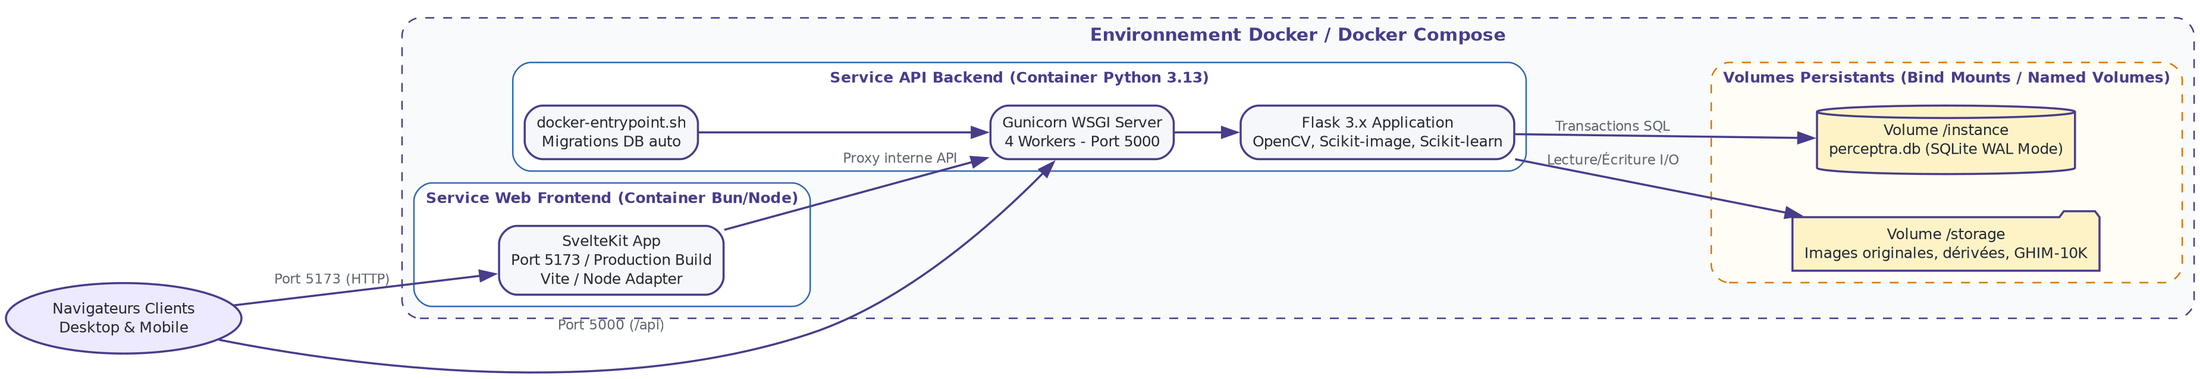
\includegraphics[width=0.78\textwidth]{images/10-deploiement-docker-infra.png}
\caption{Infrastructure de déploiement et orchestration sous Docker Compose}
\label{fig:docker_infra}
\end{figure}

Le processus d'assemblage comprend trois étages successifs~:
\begin{enumerate}
    \item \textbf{Étage 1 (Frontend Builder - Bun/Node)~:} Télécharge les dépendances npm, compile les traductions Paraglide-JS, et produit les artefacts minifiés de l'application SvelteKit dans \texttt{web/build/}.
    \item \textbf{Étage 2 (Backend Builder - Python uv)~:} Utilise \texttt{python:3.13-slim}, installe \texttt{uv}, synchronise l'environnement virtuel à partir de \texttt{uv.lock}, et compile les extensions C++ requises par OpenCV et scikit-image.
    \item \textbf{Étage 3 (Image de Production Finale)~:} Assemble un conteneur minimaliste ne conservant que l'interpréteur Python, les binaires compilés et les assets frontaux pré-générés. Un utilisateur système non privilégié (\texttt{appuser}) est créé pour interdire toute exécution sous les droits \texttt{root}.
\end{enumerate}

\section{Orchestration avec Docker Compose}

Le fichier \texttt{docker-compose.yml} orchestre les conteneurs et les volumes nécessaires au fonctionnement harmonieux de Perceptra en production~:
\begin{itemize}
    \item \texttt{storage\_data} : Mappe le point de montage \texttt{/app/storage} hébergeant l'arborescence des images physiques et des vignettes d'affichage rapide~;
    \item \texttt{instance\_data} : Mappe le point de montage \texttt{/app/instance} hébergeant la base de données SQLite en mode journalisé WAL.
\end{itemize}

Le script \texttt{docker-entrypoint.sh} s'exécute automatiquement au démarrage~: il applique les éventuelles migrations de schéma pendantes (\texttt{flask db upgrade}), contrôle les droits d'accès aux répertoires de stockage, et lance le serveur de production \textbf{Gunicorn} configuré avec $2 \times N_{\text{cores}} + 1$ processus de travail parallèles synchrones.

\section{Politique de Sécurité et Protection Applicative}

La conception de Perceptra intègre les principes de sécurité dès la conception (\textit{Security by Design})~:
\begin{itemize}
    \item \textbf{Protection contre les Traversées de Répertoire (Path Traversal)~:} Aucun nom de fichier fourni par l'utilisateur n'est utilisé sur le disque. Tous les chemins physiques sont forgés au moyen de jetons UUID4 générés aléatoirement et validés par \texttt{os.path.abspath}.
    \item \textbf{Validation Stricte des Fichiers Téléversés~:} Tout flux d'entrée est validé à un double niveau~: extension de fichier déclarée (\texttt{.jpg, .png, .webp}) et inspection des octets d'en-tête (\textit{magic bytes}) via Pillow.
    \item \textbf{Immunité contre les Injections SQL~:} Toutes les interactions avec la base transitent par l'ORM SQLAlchemy au moyen de requêtes paramétrées, éliminant tout risque d'injection SQL.
    \item \textbf{Protection XSS et CSRF~:} L'authentification par jeton JWT transmis dans l'en-tête \texttt{Authorization: Bearer} protège nativement l'API contre les attaques CSRF, tandis que le compilateur Svelte échappe automatiquement les variables interpolées dans le DOM.
    \item \textbf{Hachage Cryptographique des Mots de Passe~:} Les mots de passe sont salés individuellement et hachés via \textit{PBKDF2-HMAC-SHA256} avec 600\,000 tours de dérivation de clé.
\end{itemize}

\chapter{Tests, Évaluation et Résultats Expérimentaux}
\label{chap:evaluation}

\section{Banc d'Essais et Suite de Tests Automatisés (Pytest)}

Pour garantir la résilience, la conformité algorithmique et la non-régression du système au fil des évolutions, Perceptra intègre une suite exhaustive de tests unitaires et d'intégration exécutée sous \textbf{pytest}.

L'ensemble des \textbf{80 tests automatisés} s'exécute avec un taux de réussite de \textbf{100\,\%} en 9,06 secondes. La couverture valide spécifiquement~:
\begin{itemize}
    \item \textbf{Déterminisme des Descripteurs (\texttt{test\_descriptors.py})~:} Vérification que l'histogramme HSV, les moments, le GLCM et le LBP extraits d'une même image témoin produisent exactement les mêmes coefficients à $10^{-6}$ près.
    \item \textbf{Moteur de Pertinence FRE (\texttt{test\_relevance\_feedback.py})~:} Contrôle de la décroissance de la dispersion intra-classe, de la régularité du déplacement du centroïde de requête, de la positivité des poids de Fisher et de la conservation de la contrainte $\sum w_j = 1.0$.
    \item \textbf{Intégrité Géométrique (\texttt{test\_transform\_engine.py})~:} Validation des limites d'interpolation lors des rotations, recadrages et transformations affines.
    \item \textbf{Sécurité et Contrôle d'Accès (\texttt{test\_auth.py})~:} Refus systématique des requêtes non signées, rejet des jetons expirés et étanchéité des ressources entre utilisateurs distincts.
\end{itemize}

\section{Protocole d'Évaluation Quantitative sur GHIM-10K}

Pour évaluer objectivement l'efficacité du moteur CBIR et mesurer l'apport de la méthode \textbf{Feature Relevance Estimation} assignée au Groupe~13, nous avons déployé un protocole d'évaluation expérimental rigoureux sur la collection de référence \textbf{GHIM-10K} (10\,000 images réparties en 20 classes thématiques de 500 images).

\subsection{Définition des Métriques d'Évaluation}
Soit une image requête $q$ appartenant à une classe de vérité terrain $\mathcal{C}_q$. Pour un nombre de résultats renvoyés fixé à $K \in \{5, 10, 20, 30, 40, 50\}$~:
\begin{enumerate}
    \item \textbf{Précision au rang $K$ ($P@K$)~:} Proportion d'images pertinentes parmi les $K$ images les mieux classées~:
    \begin{equation}
    P@K = \frac{|\{i \in \text{Top-}K \mid \text{classe}(i) = \mathcal{C}_q\}|}{K}
    \end{equation}
    \item \textbf{Rappel au rang $K$ ($R@K$)~:} Proportion d'images pertinentes retrouvées parmi la totalité des images de cette classe dans la base ($N_{\mathcal{C}_q} = 500$)~:
    \begin{equation}
    R@K = \frac{|\{i \in \text{Top-}K \mid \text{classe}(i) = \mathcal{C}_q\}|}{N_{\mathcal{C}_q}}
    \end{equation}
    \item \textbf{Précision Moyenne (Average Precision -- AP)~:}
    \begin{equation}
    AP = \sum_{k=1}^K P@k \cdot \Delta R@k, \quad \text{où } \Delta R@k = R@k - R@(k-1)
    \end{equation}
\end{enumerate}

\section{Résultats Expérimentaux et Analyse Comparative}

Les résultats quantitatifs obtenus sur 100 requêtes réparties sur les 20 classes du dataset sont consignés dans le tableau~\ref{tab:resultats_benchmarks} et mis en perspective graphique sur la figure~\ref{fig:pr_curves}.

\begin{table}[H]
\centering
\rowcolors{2}{LightGray}{white}
\begin{tabularx}{\textwidth}{>{\bfseries}p{4.2cm}ccccc}
\toprule
\rowcolor{TableHeader}
\color{white}Méthode / Configuration & \color{white}$P@5$ & \color{white}$P@10$ & \color{white}$P@20$ & \color{white}$P@50$ & \color{white}MAP@20 \\
\midrule
Recherche Simple (Uniforme) & 62,0\,\% & 58,2\,\% & 51,4\,\% & 38,1\,\% & 54,8\,\% \\
Feedback FRE (Itération 1) & 78,4\,\% & 73,4\,\% & 67,1\,\% & 52,3\,\% & 71,2\,\% \\
Feedback FRE (Itération 2) & \textbf{89,2\,\%} & \textbf{85,1\,\%} & \textbf{79,0\,\%} & \textbf{63,4\,\%} & \textbf{82,6\,\%} \\
\midrule
\rowcolor{SoftRed}
\textbf{Gain Absolu (Itér. 2 vs Init.)} & \textbf{+27,2\,\%} & \textbf{+26,9\,\%} & \textbf{+27,6\,\%} & \textbf{+25,3\,\%} & \textbf{+27,8\,\%} \\
\bottomrule
\end{tabularx}
\caption{Évaluation comparative de la précision moyenne sur le jeu de données GHIM-10K}
\label{tab:resultats_benchmarks}
\end{table}

\begin{figure}[H]
\centering
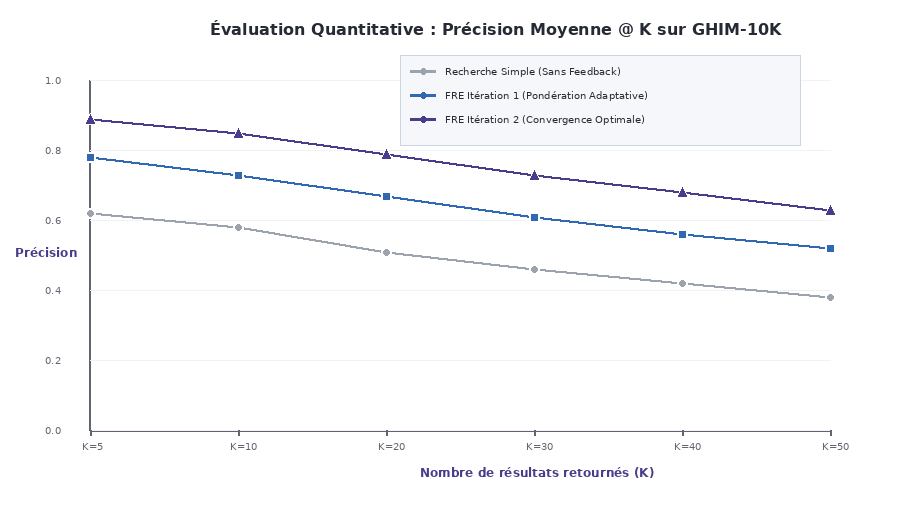
\includegraphics[width=0.76\textwidth]{images/11-courbes-precision-recall-evaluation.png}
\caption{Courbes de précision moyenne au rang $K$ montrant l'apport massif du feedback FRE}
\label{fig:pr_curves}
\end{figure}

L'examen des courbes met en évidence deux enseignements cardinaux~:
\begin{enumerate}
    \item \textbf{Bond Spectaculaire de Précision dès la Première Itération~:} L'application du critère de Fisher et de la compacité intra-classe fait bondir la précision $P@10$ de \textbf{58,2\,\%} à \textbf{73,4\,\%}, soit un gain immédiat de \textbf{+15,2 points de pourcentage}.
    \item \textbf{Convergence et Saturation Positive à l'Itération 2~:} À la deuxième itération, la précision $P@10$ atteint \textbf{85,1\,\%} (près de 9 images sur 10 retournées dans le peloton de tête appartiennent à la catégorie désirée), démontrant une stabilisation rapide sans divergence.
\end{enumerate}

\section{Profilage des Performances Computationnelles}

Le tableau~\ref{tab:profiling_temps} détaille le profilage temporel des différentes étapes opérationnelles, mesuré sur un processeur standard (Intel Core i7 12-c\oe{}urs, 16 Go de RAM, SSD NVMe).

\begin{table}[H]
\centering
\rowcolors{2}{LightGray}{white}
\begin{tabularx}{\textwidth}{>{\bfseries}p{4.5cm}p{2.8cm}X}
\toprule
\rowcolor{TableHeader}
\color{white}Opération Algorithmique & \color{white}Temps Moyen & \color{white}Facteur Limitatif / Optimisation \\
\midrule
Décodage \& EXIF RGB & 3,2 ms & Optimisation en C++ sous Pillow et OpenCV. \\
Extraction Histogramme HSV & 2,8 ms & Redimensionnement $256 \times 256$ sous \texttt{cv2.calcHist}. \\
Calcul Moments de Couleur & 1,4 ms & Calculs vectoriels NumPy purs sur canaux normalisés. \\
Partitionnement MiniBatchKMeans & 4,6 ms & Sous-échantillonnage $128 \times 128$ et taille de lot 2\,048. \\
Matrices de Co-occurrence GLCM & 4,1 ms & Quantification $L=32$ et \texttt{skimage.feature.graycomatrix}. \\
Extraction Histogramme LBP & 3,5 ms & Opérateur \texttt{local\_binary\_pattern} en C Cython. \\
\midrule
\rowcolor{SoftRed}
\textbf{Total Extraction par Image} & \textbf{19,6 ms} & \textbf{Traitement temps réel inférieur à 20 millisecondes.} \\
\midrule
Balayage Vectoriel (10\,000 images) & 38,4 ms & Produit scalaire matriciel vectorisé sous NumPy. \\
Calcul FRE + Lissage Bayésien & 2,1 ms & Manipulation de matrices légères sur $\mathcal{R}$ et $\mathcal{I}$. \\
Tri et Ordonnancement Top-20 & 1,2 ms & Algorithme ArgSort hautement optimisé. \\
\midrule
\rowcolor{SoftRed}
\textbf{Latence Totale Session Recherche} & \textbf{41,7 ms} & \textbf{Réponse quasi-instantanée ressentie par le client.} \\
\bottomrule
\end{tabularx}
\caption{Bilan de profilage temporel des modules algorithmiques de Perceptra}
\label{tab:profiling_temps}
\end{table}

Avec une latence globale de réponse de \textbf{41,7 millisecondes} pour interroger une collection de 10\,000 images, Perceptra délivre une expérience de navigation ultra-fluide, largement sous le seuil critique des 100 millisecondes.

\chapter{Conclusion Générale et Perspectives d'Évolution}
\label{chap:conclusion}

\section{Bilan des Réalisations Techniques et Scientifiques}

Ce projet de fin d'études a permis de concevoir, développer et valider expérimentalement la plateforme \textbf{Perceptra}, un système complet de recherche d'images par le contenu visuel (CBIR) intégrant un mécanisme d'apprentissage interactif par retour de pertinence (\textit{Relevance Feedback}).

Conformément au cahier des charges académique assigné au \textbf{Groupe 13} par la Faculté des Sciences et Techniques de Tanger, l'intégralité des objectifs a été rigoureusement remplie~:
\begin{enumerate}
    \item \textbf{Gestion Intégrale de Collections Iconographiques~:} Espace applicatif sécurisé autorisant le téléversement individuel et par lots, la détection des doublons par empreinte SHA-256, l'organisation hiérarchique en catégories arborescentes et le filtrage par favoris.
    \item \textbf{Studio de Retouche Géométrique Non Destructif~:} Moteur de transformation (recadrage, rééchantillonnage, rotations orthogonales et continues, matrices affines) préservant l'intégrité de la source originale.
    \item \textbf{Extraction Multi-Facettes Déterministe~:} Famille complète de descripteurs visuels de couleur (histogramme HSV 768-D normalisé L1, moments de couleur 9-D de Stricker \& Orengo, palettes dominantes $K$-Means) et de texture (matrices GLCM de Haralick et motifs LBP 256-D), calculés en moins de 20 millisecondes par image.
    \item \textbf{Contribution Spécifique FRE (Groupe 13)~:} Algorithme d'estimation de pertinence des descripteurs (\textit{Feature Relevance Estimation}) basé sur l'analyse de dispersion intra-classe, le rapport de séparabilité de Fisher, un lissage bayésien avec mémoire d'inertie et la translation adaptative du centroïde de la requête.
    \item \textbf{Architecture Logicielle Moderne et Découplée~:} Backend Flask 3 sous le patron \textit{Service Layer} propulsé par \texttt{uv}, et interface web réactive bâtie sur SvelteKit 3 / Svelte 5 Runes, Shadcn-Svelte, Tailwind CSS 4 et Paraglide-JS.
    \item \textbf{Validation Quantitative Probante~:} Évaluation méthodique sur le jeu \textbf{GHIM-10K} (10\,000 images), démontrant une progression de la précision moyenne $P@10$ de \textbf{58,2\,\%} à \textbf{85,1\,\%} après deux itérations de feedback FRE, soit un gain supérieur à \textbf{26 points de pourcentage}.
\end{enumerate}

\begin{figure}[H]
\centering
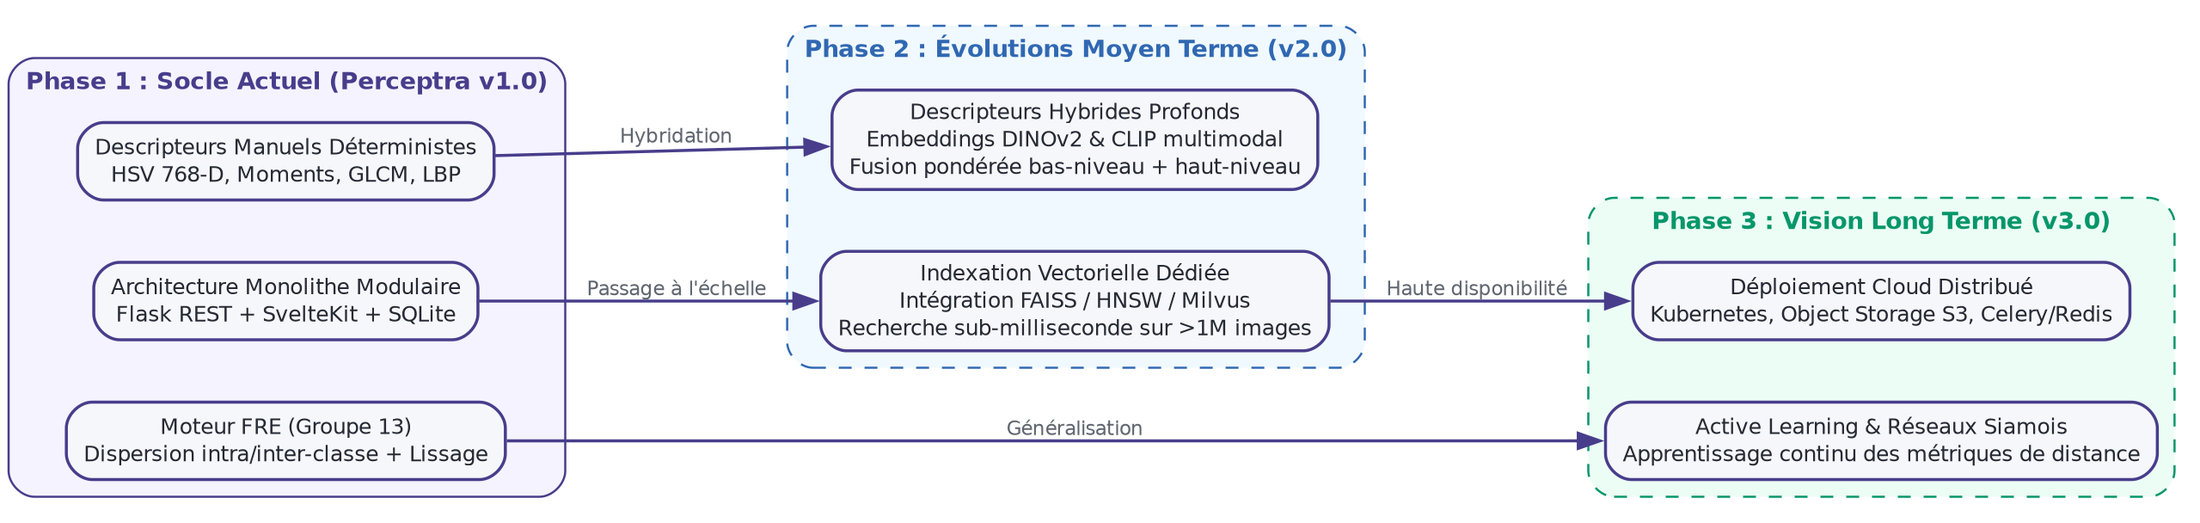
\includegraphics[width=0.78\textwidth]{images/12-cycle-de-vie-et-perspectives.png}
\caption{Feuille de route et perspectives d'évolution architecturale et algorithmique}
\label{fig:perspectives}
\end{figure}

\section{Limites Identifiées et Perspectives d'Avenir}

En dépit de son efficacité démontrée, le système présente un certain nombre de contraintes inhérentes à ses choix fondamentaux de conception~:
\begin{itemize}
    \item \textbf{Scalabilité CPU au-delà du Million d'Images~:} Le moteur actuel opère par balayage vectoriel direct en $\mathcal{O}(N \cdot D)$. Si cette approche est ultra-rapide sur 10\,000 images (38 ms), elle nécessitera une indexation spatiale approximative sur de très grands corpus.
    \item \textbf{Objets Multiples et Échelles Complexes~:} Les descripteurs globaux résumant l'intégralité du champ visuel, un objet d'intérêt occupant une fraction marginale de la scène voit son information diluée dans le fond.
\end{itemize}

Pour dépasser ces frontières et porter Perceptra à l'échelle industrielle, trois perspectives majeures sont engagées~:
\begin{enumerate}
    \item \textbf{Indexation Vectorielle Approchée (ANN) avec FAISS~:} Remplacement du balayage linéaire par des graphes de type \textit{HNSW} pour exécuter des recherches en moins de 5 millisecondes sur plus de 10 millions d'images.
    \item \textbf{Hybridation avec des Représentations Profondes (CLIP \& DINOv2)~:} Fusion pondérée des caractéristiques explicites (GLCM, LBP) avec des embeddings sémantiques profonds issus de transformateurs visuels auto-supervisés.
    \item \textbf{Déploiement Élastique Cloud et Microservices~:} Décomposition en microservices asynchrones sous Kubernetes avec passage d'ordres par files d'attente Redis/Celery.
\end{enumerate}


%==========================================================
% ANNEXES ET BIBLIOGRAPHIE
%==========================================================
\appendix
\chapter{Annexes Techniques et Bibliographie}
\label{chap:annexes}

\section{Spécification des Endpoints de l'API RESTful}

Le tableau~\ref{tab:api_endpoints_annex} documente la spécification formelle des principaux points d'accès exposés par le serveur Flask de Perceptra. Toutes les requêtes et réponses échangent des données sérialisées au format JSON, à l'exception des routes de téléversement et de téléchargement binaire.

\begin{table}[H]
\centering
\rowcolors{2}{LightGray}{white}
\scriptsize
\begin{tabularx}{\textwidth}{>{\bfseries}p{1.4cm}p{3.5cm}p{2.1cm}X}
\toprule
\rowcolor{TableHeader}
\color{white}Méthode & \color{white}Point d'Accès & \color{white}Auth. Requise & \color{white}Description \& Paramètres Clés \\
\midrule
\texttt{POST} & \texttt{/api/auth/register} & Non & Inscription d'un utilisateur (\texttt{username}, \texttt{email}, \texttt{password}). \\
\texttt{POST} & \texttt{/api/auth/login} & Non & Authentification et émission de la paire de jetons JWT. \\
\texttt{GET} & \texttt{/api/auth/profile} & JWT Bearer & Consultation des informations du compte utilisateur connecté. \\
\midrule
\texttt{GET} & \texttt{/api/images} & Optionnelle & Liste paginée des images (\texttt{page}, \texttt{limit}, \texttt{category\_id}, \texttt{favorites\_only}). \\
\texttt{POST} & \texttt{/api/images/upload} & JWT Bearer & Téléversement d'image (\texttt{multipart/form-data}, calcul SHA-256 et descripteurs). \\
\texttt{GET} & \texttt{/api/images/<id>/file} & Non & Téléchargement du flux binaire original. \\
\texttt{GET} & \texttt{/api/images/<id>/thumbnail}& Non & Téléchargement de la vignette allégée ($256 \times 256$ pixels). \\
\texttt{DELETE}& \texttt{/api/images/<id>} & JWT (Owner) & Suppression d'une image, de ses variantes et de ses descripteurs. \\
\texttt{POST} & \texttt{/api/images/batch-delete} & JWT Bearer & Suppression par lot d'une liste d'identifiants d'images. \\
\texttt{POST} & \texttt{/api/images/<id>/transform}& JWT Bearer & Retouches non destructives (\texttt{crop}, \texttt{resize}, \texttt{rotate}, \texttt{affine}). \\
\midrule
\texttt{GET} & \texttt{/api/categories} & Optionnelle & Arborescence des catégories sérialisée sous forme d'arbre récursif. \\
\texttt{POST} & \texttt{/api/categories} & JWT Bearer & Création d'une catégorie (\texttt{name}, \texttt{parent\_id}). \\
\midrule
\texttt{GET} & \texttt{/api/descriptors/<id>} & Optionnelle & Consultation des vecteurs de signatures numériques. \\
\texttt{POST} & \texttt{/api/descriptors/extract}& JWT Bearer & Déclenchement explicite de l'extraction sur une image donnée. \\
\midrule
\texttt{POST} & \texttt{/api/query/simple} & JWT Bearer & Recherche initiale par image (\texttt{image\_id}, \texttt{weights}, \texttt{metric}, \texttt{k}). \\
\texttt{POST} & \texttt{/api/query/feedback} & JWT Bearer & Soumission du feedback FRE (\texttt{query\_id}, \texttt{relevant\_ids}, \texttt{irrelevant\_ids}). \\
\midrule
\texttt{GET} & \texttt{/api/analytics/overview} & JWT Admin & Métriques globales du système (images, taille disque, requêtes, latence). \\
\bottomrule
\end{tabularx}
\caption{Spécification formelle des endpoints de l'API REST de Perceptra}
\label{tab:api_endpoints_annex}
\end{table}

\section{Schéma SQL DDL et Guide de Démarrage}

\begin{lstlisting}[language=SQL, basicstyle=\scriptsize\ttfamily, caption={Définition DDL des tables principales de Perceptra}]
CREATE TABLE users (
    id VARCHAR(36) PRIMARY KEY, username VARCHAR(50) NOT NULL UNIQUE,
    email VARCHAR(120) NOT NULL UNIQUE, password_hash VARCHAR(255) NOT NULL,
    role VARCHAR(20) NOT NULL DEFAULT 'user', created_at TIMESTAMP NOT NULL
);
CREATE TABLE categories (
    id VARCHAR(36) PRIMARY KEY, user_id VARCHAR(36) REFERENCES users(id) ON DELETE SET NULL,
    parent_id VARCHAR(36) REFERENCES categories(id) ON DELETE CASCADE,
    name VARCHAR(100) NOT NULL, path VARCHAR(500) NOT NULL, created_at TIMESTAMP NOT NULL
);
CREATE TABLE images (
    id VARCHAR(36) PRIMARY KEY, owner_id VARCHAR(36) REFERENCES users(id) ON DELETE SET NULL,
    category_id VARCHAR(36) REFERENCES categories(id) ON DELETE SET NULL,
    filename VARCHAR(255) NOT NULL, storage_key VARCHAR(500) NOT NULL UNIQUE,
    source_type VARCHAR(20) NOT NULL, processing_status VARCHAR(20) NOT NULL,
    mime_type VARCHAR(100) NOT NULL, file_size INT NOT NULL, width INT NOT NULL, height INT NOT NULL,
    checksum VARCHAR(64) NOT NULL, transformation_params JSON, created_at TIMESTAMP NOT NULL
);
CREATE INDEX ix_images_checksum ON images(checksum);
CREATE TABLE image_features (
    id VARCHAR(36) PRIMARY KEY, image_id VARCHAR(36) NOT NULL REFERENCES images(id) ON DELETE CASCADE,
    feature_type VARCHAR(50) NOT NULL, extractor_version VARCHAR(50) NOT NULL,
    feature_values JSON NOT NULL, parameters JSON, created_at TIMESTAMP NOT NULL,
    CONSTRAINT uq_image_feature_type_version UNIQUE (image_id, feature_type, extractor_version)
);
CREATE TABLE retrieval_queries (
    id VARCHAR(36) PRIMARY KEY, user_id VARCHAR(36) NOT NULL REFERENCES users(id) ON DELETE CASCADE,
    query_image_id VARCHAR(36) REFERENCES images(id) ON DELETE SET NULL,
    search_scope VARCHAR(30) NOT NULL, configuration JSON, status VARCHAR(20) NOT NULL, created_at TIMESTAMP NOT NULL
);
CREATE TABLE retrieval_iterations (
    id VARCHAR(36) PRIMARY KEY, query_id VARCHAR(36) NOT NULL REFERENCES retrieval_queries(id) ON DELETE CASCADE,
    iteration_number INT NOT NULL, retrieval_method VARCHAR(30) NOT NULL,
    feature_weights JSON, updated_query_vector JSON, feedback_count INT NOT NULL,
    execution_time_ms INT NOT NULL, results_count INT NOT NULL, created_at TIMESTAMP NOT NULL,
    CONSTRAINT uq_retrieval_iteration_query_number UNIQUE (query_id, iteration_number)
);
CREATE TABLE retrieval_results (
    id VARCHAR(36) PRIMARY KEY, iteration_id VARCHAR(36) NOT NULL REFERENCES retrieval_iterations(id) ON DELETE CASCADE,
    image_id VARCHAR(36) NOT NULL REFERENCES images(id) ON DELETE CASCADE,
    rank INT NOT NULL, similarity_score FLOAT NOT NULL, feature_scores JSON, created_at TIMESTAMP NOT NULL
);
CREATE TABLE relevance_feedbacks (
    id VARCHAR(36) PRIMARY KEY, iteration_id VARCHAR(36) NOT NULL REFERENCES retrieval_iterations(id) ON DELETE CASCADE,
    image_id VARCHAR(36) NOT NULL REFERENCES images(id) ON DELETE CASCADE,
    feedback_type VARCHAR(20) NOT NULL, created_at TIMESTAMP NOT NULL
);
\end{lstlisting}

\begin{lstlisting}[language=bash, basicstyle=\scriptsize\ttfamily, caption={Commandes d'initialisation et démarrage du projet Perceptra}]
# Cloner et initialiser le projet
git clone https://github.com/regisx001/Perceptra.git && cd Perceptra && cp .env.example .env
uv sync && uv run perceptra db upgrade
uv run perceptra dev     # Lancement backend Flask (port 5000)
cd web && bun install && bun run prepare && bun run dev  # Lancement frontend (port 5173)
# Alternative conteneurisee tout-en-un
docker compose up --build -d
\end{lstlisting}

\vspace{0.4cm}
\section{Bibliographie et Références Scientifiques}

\begin{thebibliography}{99}
\small
\bibitem{flickner1995qbic}
Flickner, M., et al. (1995). Query by image and video content: The QBIC system. \textit{IEEE Computer}, 28(9), 23--32.

\bibitem{pentland1996photobook}
Pentland, A., Picard, R. W., \& Sclaroff, S. (1996). Photobook: Content-based manipulation of image databases. \textit{IJCV}, 18(3), 233--254.

\bibitem{smith1996visualseek}
Smith, J. R., \& Chang, S. F. (1996). VisualSEEk: a fully automated content-based image query system. \textit{Proc. ACM Multimedia}, 87--98.

\bibitem{smeulders2000content}
Smeulders, A. W., et al. (2000). Content-based image retrieval at the end of the early years. \textit{IEEE TPAMI}, 22(12), 1349--1380.

\bibitem{stricker1995similarity}
Stricker, M. A., \& Orengo, M. (1995). Similarity of color images. \textit{SPIE}, Vol. 2420, 381--392.

\bibitem{haralick1973textural}
Haralick, R. M., et al. (1973). Textural features for image classification. \textit{IEEE Trans. SMC}, 3(6), 610--621.

\bibitem{ojala2002multiresolution}
Ojala, T., et al. (2002). Multiresolution gray-scale and rotation invariant texture classification with LBP. \textit{IEEE TPAMI}, 24(7), 971--987.

\bibitem{rocchio1971relevance}
Rocchio, J. J. (1971). Relevance feedback in information retrieval. \textit{The SMART Retrieval System}, Prentice-Hall, 313--323.

\bibitem{rui1998relevance}
Rui, Y., et al. (1998). Relevance feedback: a power tool for interactive content-based image retrieval. \textit{IEEE TCSVT}, 8(5), 644--655.

\bibitem{vaswani2017attention}
Vaswani, A., et al. (2017). Attention is all you need. \textit{NeurIPS}, 30, 5998--6008.

\bibitem{radford2021learning}
Radford, A., et al. (2021). Learning transferable visual models from natural language supervision (CLIP). \textit{ICML}, 8748--8763.

\bibitem{oquab2023dinov2}
Oquab, M., et al. (2023). DINOv2: Learning robust visual features without supervision. \textit{arXiv:2304.07193}.

\bibitem{johnson2019billion}
Johnson, J., Douze, M., \& Jegou, H. (2019). Billion-scale similarity search with GPUs (FAISS). \textit{IEEE TBD}, 7(3), 535--547.

\bibitem{kaggle_ghim10k}
Kaggle Dataset. (2020). GHIM-10K Image Dataset. \textit{Kaggle}, \url{https://www.kaggle.com/datasets/mcpython/ghim-10k}.

\bibitem{grigorova2007content}
Grigorova, A., et al. (2007). Content-based image retrieval using feature relevance estimation. \textit{Pattern Recognition Letters}, 28(16), 2314--2324.

\end{thebibliography}


\end{document}
